\documentclass[8pt,a4paper]{article}

\usepackage{atbegshi}
\AtBeginShipoutFirst{\special{pdf:tounicode EUC-UCS2}}


%空白の設定
\usepackage{geometry}
\geometry{left=20truemm, right=20truemm, top=15truemm, bottom=20truemm}


%行間の設定
\renewcommand{\baselinestretch}{1.1}

\makeatletter
\newcommand{\figcaption}[1]{\def\@captype{figure}\caption{#1}}
\newcommand{\tblcaption}[1]{\def\@captype{table}\caption{#1}}
\makeatother
%コマンドの定義
\newcommand{\pcl}{\partial}
\newcommand{\bsm}{\boldsymbol}
\newcommand{\bm}{\boldsymbol}
\newcommand{\tr}{\mathrm{tr}}
\newcommand{\udl}{\underline}

\usepackage[nottoc]{tocbibind} 
\usepackage{booktabs}
\usepackage[dvipdfmx]{graphicx}
\usepackage[dvipdfmx]{color}
\usepackage{amsmath, amssymb}
\usepackage{txfonts}
\usepackage{wrapfig}
\usepackage{ascmac}
\usepackage{booktabs}
\usepackage{tabularx}
\usepackage{url}
\usepackage{color}
\usepackage{scalerel}
\usepackage{subfigure}
\usepackage{listings,jlisting}
\usepackage{comment}
\usepackage{tabularx}
\usepackage{longtable}
\usepackage{here}
\begin{comment}
\lstset{ 
basicstyle=\ttfamily\scriptsize,
  commentstyle=\textit,
  classoffset=1,
  keywordstyle=\bfseries,
  frame=tRBl,
  framesep=5pt,
  showstringspaces=false,
  numbers=left,
  stepnumber=1,
  numberstyle=\tiny,
  tabsize=2
}
\end{comment}

\definecolor{identifier}{rgb}{0.611, 0.862, 0.996}  % LightBlue (変数)
\definecolor{comment}{rgb}{0.415, 0.600, 0.333}     % DeepGreen (コメント)
\definecolor{keyword1}{rgb}{0.768, 0.521, 0.749}    % Purple    (予約語)
\definecolor{keyword2}{rgb}{0.862, 0.862, 0.666}    % Yellow    (関数名)
\definecolor{keyword3}{rgb}{0.2, 0.8, 1}            % Blue      (大域変数)
\definecolor{keyword4}{rgb}{0.854, 0.439, 0.839}    % Pink      (定数)
\definecolor{string}{rgb}{0.847, 0.560, 0.458}      % Orange    (文字列)

\lstset{
language={C},
backgroundcolor={\color[gray]{.85}},
basicstyle={\small\ttfamily},
identifierstyle={\small},
commentstyle={\small\ttfamily \color{comment}},
keywordstyle={\small\bfseries \color[rgb]{0,0,0.7}},
ndkeywordstyle={\small},
stringstyle={\small\ttfamily \color{keyword4}},
frame={tb},
breaklines=true,
columns=[l]{fullflexible},
numbers=left,
xrightmargin=0zw,
xleftmargin=3zw,
numberstyle={\scriptsize},
stepnumber=1,
numbersep=1zw,
morecomment=[l]{//}
}

\DeclareMathOperator*{\assem}{\scalerel*{\textsf{A}}{\sum}}
%\usepackage[refeq, refpage, japanese]{nomencl}
%\makenomenclature

\setcounter{tocdepth}{4}
\setcounter{secnumdepth}{3}
\newcommand{\todayd}{\the\year/\the\month/\the\day}


\begin{document} 

\begin{center}
	{\Large BBFE mlflowのマニュアル} \\
\end{center}

\tableofcontents

\newpage
\section{非圧縮性粘性流れの計算}
\subsection{支配方程式}
非圧縮性粘性流れの運動方程式は以下のNavier-Stokes方程式によって記述される。
\begin{equation}
\label{fluid-ns}
\rho \frac{D\bm{u}}{Dt} = - \nabla p + \mu \nabla^{2} \bm{u} + \bm{f}
\end{equation}
ここで、$\rho$は流体の密度、$\bm{u}$は流体の速度ベクトル、$p$は流体の圧力、$\mu$は流体の粘性係数、$\bm{f}$は外力ベクトルを表す。
また、非圧縮性流れにおける連続の式は以下のように表される。
\begin{equation}
\label{fluid-continuum}
\nabla \cdot u = 0
\end{equation}

流体は非圧縮性粘性を仮定しているため、Navier-Stokes方程式(\ref{fluid-ns})と非圧縮性の連続の式(\ref{fluid-continuum})を解く。

\subsection{Fractional step法}
流体解析プログラムでは、流体を解く手法として分離型解法の一つであるFractional Step法を使用する。
Navier-Stokes方程式(\ref{fluid-ns})において、外力項を省略し、両辺を流体の密度$\rho$で割って無次元化したNavier-Stokes方程式は以下の式(\ref{fs-ns})のように記述される。ここではEinsteinの縮約記法を用いる。
\begin{equation}
\label{fs-ns}
	\frac{u^{n+1}_i - u^{n}_i}{\Delta t} + u^{n}_i \frac{\partial u^{n}_i}{\partial x_j}
	+ \frac{\partial p^{n+1}}{\partial x_i} - \frac{1}{\mathrm{Re}} \frac{\partial^{2} u^{n}_i}{\partial x^{2}_j} = 0
\end{equation}
ここで$u^{n}_{i}$は$n$ステップ目における$i$方向の流速、$\mathrm{Re}$はレイノルズ数を表す。

また、$n+1$ステップ目を満たす連続の式は以下の式(\ref{fs-continuum})ように記述される。
\begin{equation}
\label{fs-continuum}
	\frac{\partial u_{i}^{n+1}}{\partial x_{i}}=0
\end{equation}

式(\ref{fs-continuum})の発散を取り、式(\ref{fs-ns})に代入すると以下の圧力Poisson方程式(\ref{fs-poisson})が導かれる。
\begin{equation}
\label{fs-poisson}
	\frac{\partial^2 p^{n+1}}{\partial x^{2}_i} = \frac{1}{\Delta t} \frac{\partial \tilde{u}_i}{\partial x_{i}}
\end{equation}

ここで$\tilde{u}_{i}$は中間流速であり、以下の式(\ref{fs-midvel})で記述される。
\begin{equation}
\label{fs-midvel}
	\tilde{u}_{i} = u_{i}^{n} - \Delta t
	\left(u_{j}^{n} \frac{\partial u_{i}^{n}}{\partial x_{j}} 
	- \frac{1}{\mathrm{Re}} \frac{\partial^{2} u_{i}^{n}}{\partial x_{j}^{2}}\right)
\end{equation}

圧力Poisson方程式(\ref{fs-poisson})を解いて求めた$n+1$ステップ目の圧力$p^{n+1}$を使って速度を修正することで$n+1$ステップ目の流速$u^{n+1}_{i}$を次式(\ref{fs-correct})により求める。
\begin{equation}
\label{fs-correct}
	u^{n+1}_i=\tilde{u}_i - \Delta t \frac{\partial p^{n+1}}{\partial x_i}
\end{equation}

\subsection{SUPG法による安定化有限要素法の定式化}
Navier-Stokes方程式を数値的に解く時、移流項が卓越する場合には数値的な不安定性が生じるという問題がある。
有限要素法において、移流項による数値不安定性を防ぐ方法として、SUPG(Streamline Upwind/Petrov-Galerkin)法が提案された。SUPG法は、移流項の重みを変化させることで、流れの流線方向にのみ安定化させることができる手法である。

Fractional Step法を用いて定式化した式(\ref{fs-midvel})・(\ref{fs-poisson})・(\ref{fs-correct})にSUPG法を適用する。
Galerkin法に基づいて、流速の重み関数$w_{i}$、流速$u_{i}$、中間流速$\tilde{u}_{i}$、圧力の重み関数$q$、圧力$p$を次の式(\ref{supg-fs})ように近似する。
\begin{equation}
\label{supg-fs}
	\begin{split}
		w_{i}^{h}=&N_{\alpha}^{e} w_{i\alpha}^{e},\; u_{i}^{h}=N_{\alpha}^{e} u_{i\alpha}^{e},\; 
		\tilde{u}_{i}^{h}=N_{\alpha}^{e} \tilde{u}_{i\alpha}^{e}, \\
		q^{h}=&L_{\alpha}^{e} q_{\alpha}^{e}, \; p^{h}=L_{\alpha}^{e} p_{\alpha}^{e} \\
	\end{split}
\end{equation}
ここで$u_{i\alpha}^{e}$、$\tilde{u}_{i\alpha}^{e}$、$p_{\alpha}$はそれぞれ流速、中間流速、圧力の節点値である。また、$N_{\alpha}$、$L_{\alpha}$はそれぞれ流速場と圧力場に対する形状関数である。$e$は要素のインデックスを表す。

中間流速を求める式は以下の式(\ref{supg-midvel})の通り。
\begin{equation}
\label{supg-midvel}
	\begin{split}
		\int_{\Omega} w_{i}\left( \frac{\tilde{u}-v^{n}_i}{\Delta t} + u^{n}_{j} \frac{\partial u^{n}_{i}}{\partial x_{j}}\right) \; d\Omega \;+ 
		\int_{\Omega} \frac{1}{\mathrm{Re}} \frac{\partial w_{i}}{\partial x_{j}} \frac{\partial u^{n}_{i}}{\partial x_{j}} \; d\Omega \;+& \\
		\sum_{e=1}^{M} \int_{\Omega_{e}} \tau_{m} u_{j}^{n} \frac{\partial w_{i}^{h}}{\partial x_{j}} \left( \frac{\tilde{u_{i}} - u_{i}^{n}}{\Delta t} + u_{j}^{n} \frac{\partial u_{i}^{n}}{\partial x_{j}} - \frac{1}{Re} \frac{\partial^{2} u_{i}^{n}}{\partial x_{j}^{2}}\right) \; d\Omega \;=& 
		\int_{\Gamma_{h}} w_{i}\frac{1}{\mathrm{Re}} \frac{\partial u_{i}}{\partial x_{j}}n_{j} \;d\Gamma
	\end{split}
\end{equation}

ここで$e$は要素のインデックス、$M$は全要素数、$\Omega_{e}$は要素領域、$\tau_{m}$は安定化パラメータであり、要素での安定化パラメータ$\tau_{m}^{e}$は次式(\ref{supg-tau})で与えられる。
\begin{equation}
\label{supg-tau}
	\tau_{m}^{e}=\left[ \left(\frac{2}{\Delta t}\right)^{2} + \left(\frac{2||\bm{u}||}{h_{e}}\right)^{2} + \left(\frac{4}{\mathrm{Re_{v}} h_{e}^{2}}\right)^{2}\right]^{-1/2}
\end{equation}
$\Delta t$は時間刻み幅、$\bm{u}$は流速、$h_e$は要素サイズ、$\mathrm{Re_u}$は要素レイノルズ数である。

圧力ポアソン方程式は以下の式(\ref{supg-poisson})のようになる。
\begin{equation}
\label{supg-poisson}
	\int_{\Omega} q \frac{\partial^{2}p^{n+1}}{\partial x_{i}^{2}} \; d\Omega = 
	\frac{1}{\Delta t} \int_{\Omega} q \frac{\partial \tilde{u}_{i}}{\partial x_{i}} \; d\Omega
\end{equation}

速度の修正の式は以下の式(\ref{supg-correct})のようになる。
\begin{equation}
\label{supg-correct}
	\int_{\Omega} w_{i}u_{i}^{n+1} \; d\Omega = \int_{\Omega} w_{i} \tilde{u}_{i} \; d\Omega
	- \Delta t \int_{\Omega} w_{i} \frac{\partial p^{n+1}}{\partial x_{i}} d\Omega
\end{equation}

式(\ref{supg-midvel})・(\ref{supg-poisson})・(\ref{supg-correct})を行列で表すとそれぞれ式(\ref{matrix-midvel})・(\ref{matrix-poisson})・(\ref{matrix-correct})になる。ただし、式(\ref{supg-poisson})に対しては部分積分を行う。
\begin{equation}
\label{matrix-midvel}
	( \bm{M} + \bm{M}_{s} ) \frac{\tilde{\bm{u}}_i - \bm{u}_{i}^{n}}{\Delta t} + ( \bm{A} + \bm{A}_s ) \bm{u}_{i}^{n} + \bm{D} \bm{u}_{i}^{n} = 0
\end{equation}

\begin{equation}
\label{matrix-poisson}
	-\bm{G} \bm{p}^{n+1} = \frac{1}{\Delta t} \bm{C} \tilde{\bm{u}}_{i} - \bm{G}_{\Gamma}
\end{equation}

\begin{equation}
\label{matrix-correct}
	\bm{M} \bm{u}_{i}^{n+1} = \bm{M} \tilde{\bm{u}}_{i} - \Delta t \bm{C} \bm{p}^{n+1}
\end{equation}

\newpage
\section{レベルセット法による自由表面流れの計算}
自由表面流れとして界面捕捉法の手法であるレベルセット法にを用いた自由表面流れ解析手法について述べる。

\subsection{支配方程式}
レベルセット法による自由表面流れの支配方程式は、
Navier-Stokes方程式(\ref{fluid-ns})と連続の式(\ref{fluid-continuum})で表される。

界面捕捉法では解析メッシュは固定メッシュを用いるため、界面を間接的に表現するための関数(界面関数)を導入する。
界面の支配方程式は以下の移流方程式(\ref{ls-eq})で表される。
\begin{equation}
\label{ls-eq}
	\frac{\partial \phi}{\partial t} + \bm{u} \cdot \nabla \phi = 0 \quad in \quad \Omega
\end{equation}
ここで、$\phi$が界面関数、$\bm{u}$は速度である。
式(\ref{ls-eq})に対してSUPG法に基づく安定化有限要素法を適用し解くことでレベルセット関数が求められる。

\subsection{SUPG法による安定化有限要素法}
式(\ref{ls-eq})にSUPG法を適用すると以下の式(\ref{ls-supg})が得られる。
\begin{equation}
\label{ls-supg}
		\begin{split}
		\int_{\Omega} \psi^{h}\left( \frac{\partial \phi}{\partial t} + \bm{u}^{n} \cdot \nabla \phi^{h} \right) \; d\Omega \;+& 
		\sum^{n_el}_{e=1} \int_{\Omega_{e}} \tau_{\phi} \bm{u}^{h} \cdot \nabla \psi^{h} \left( \frac{\partial \phi^{h}}{\partial t} + \bm{u}^{h} \cdot \nabla \phi^{h} \right) \; d\Omega \\
		+& \sum^{n_el}_{e=1} \int_{\Omega_{e}} \tau_{LSIC} \nabla \psi^{h} \cdot \nabla \phi^{h} \; d\Omega = 0
	\end{split}
\end{equation}
ここで$\tau_\phi$, $\tau_{LSIC}$はそれぞれ式(\ref{ls-tau_phi}), (\ref{ls-tau_LSIC})に示すSUPG項と衝撃捕捉項のパラメータである。
\begin{equation}
\label{ls-tau_phi}
	\tau_{\phi} = \left[ \left(\frac{2}{\Delta t} \right)^2 + \left(\frac{2 \| \bm{u}^{h} \|}{h_{e}} \right)^2 \right]^{-1/2}
\end{equation}

\begin{equation}
\label{ls-tau_LSIC}
	\tau_{LSIC} = \frac{h_{e}}{2} \| \bm{u}^{h} \|
\end{equation}

\subsection{レベルセット法}
レベルセット法は、自由表面の位置をレベルセット関数と呼ばれる界面からの距離関数を用いて定義する。
自由表面流れにおけるレベルセット関数の定義は、自由表面上(界面)で0、自由表面から液体の方向に対して正、気体の方向に対して負であるものとする。
レベルセット関数の等距離である性質としては次式(\ref{ls-charcter})を満たすものとする。
\begin{equation}
\label{ls-charcter}
	| \nabla \phi | = 1
\end{equation}

レベルセット法は、任意の時間におけるレベルセット関数$\phi$から次式(\ref{ls-heaviside})に示す近似Heaviside関数$H_{D}$を用いることにより界面近傍の平滑化を行う。
\begin{equation}
\label{ls-heaviside}
	H_{D} = 0.5 \cdot \max \left[-1.0, \min \left(1.0, \frac{\phi}{D} + \frac{1}{\pi} sin\left(\frac{\pi \phi}{D}\right)\right) \right]
\end{equation}

\subsection{表面張力}
表面張力$\bm{f}_{fs}$とすると、CSF(Continuum Surface Force)モデルにより次式(\ref{sf-eq})のように算定できる。
\begin{equation}
\label{sf-eq}
	\bm{f}_{fs} = \sigma \kappa \nabla \phi
\end{equation}

ここで界面の曲率$\kappa$と法線方向$\bm{n}_{s}$は以下の式(\ref{sf-nv}), (\ref{sf-kappa})のように表される。
\begin{equation}
\label{sf-nv}
	\bm{n}_{s} = \frac{\nabla \phi}{| \nabla \phi |}
\end{equation}

\begin{equation}
\label{sf-kappa}
	\kappa = - \nabla \cdot \bm{n}_{s}
\end{equation}
式(\ref{sf-eq})で求められた表面張力$\bm{f}_{fs}$はNavier-Stokes方程式(\ref{fluid-ns})の体積力として作用させる。

ここで、表面張力の計算式には2階微分が含まれるので線形近似では要素内で値が0になってしまう問題がある。
L2プロジェクションによる計算\cite{Nagrath2003}や、1階微分の値を各節点に振り分けてから1次要素で補間する方法\cite{Matsumoto2006}, \cite{Shi2019}が提案されている。
今回は、1階微分の値を各節点に振り分けてから1次要素で補間する方法で計算した。

\newpage
\section{ソースコード解説}
ここでは、bbfe\_mflowのに含まれているプログラムのうち自由表面流れ解析の実装を中心に解説する。

\subsection{プログラムの構成}
自由表面流れ解析プログラムが実装されているディレクトリ構成とファイルを以下に示す。

\begin{itemize}
	\item FE\_solvers : 種々の問題のソルバーが存在するディレクトリ
  \begin{itemize}
    \item mlflow\_fs : 自由表面流れ解析の実装ファイルをまとめたディレクトリ
    \begin{itemize}
    	\item mlflow\_fs.c : 自由表面流れを計算するmain関数を含むファイル
    	\item mlflow\_fs.h : mlflow\_fs.cの関数のヘッダーファイル
    	\item mlflow\_core.c:節点が持つ流速・密度・粘性・レベルセット関数などの値の更新やレベルセット関数のヘビサイド関数への変換などの基本的な計算をする関数群のファイル
    	\item mlflow\_core.h : mlflow\_core.cの関数のヘッダーファイル
    	\item mlflow\_element.c : 自由表面流れの支配方程式の有限要素法により解くときの行列ベクトルを計算する関数群のファイル
    	\item mlflow\_element.h : mlflow\_element.cの関数のヘッダーファイル
    \end{itemize}
  \end{itemize}
\end{itemize}

\subsection{mlflow\_fs.c}
\subsubsection{main関数}
まずmlflow\_fs.cのmain関数を以下に示す。
時間ステップごとのforループの中で、
最初にmonolisの行列やベクトルの値の初期化やコピーにより値の準備を行い、
printfで"update density and viscosity step"と出力している部分が、
前のステップで更新したレベルセット関数をもとに、密度と粘性係数の分布を再計算し更新する部分である。
printfで"prediction step", "pressure Poisson eq.", "Correction step"と出力している部分が、
fractional step法におけるそれぞれの計算部分である。
"levelset function convection step"とprintfで出力しているところからレベルセット関数の移流方程式の計算が始まる。
\begin{lstlisting}[caption = mlflow\_fs.cのmain関数のレベルセット関数の計算部分抜粋]
int main(
		int   argc,
		char* argv[])
{
 
	/* ~初期化部分の記載省略~ */

	/****************** solver ********************/
	double t = 0.0;
	int step = 0;
	int file_num = 0;
	output_files(&sys, file_num, t);
	while (t < sys.vals.finish_time) {
		t += sys.vals.dt;
		step += 1;

		printf("\n%s ----------------- step %d ----------------\n", CODENAME, step);

		BBFE_sys_monowrap_copy_mat(&(sys.mono_ppe0) , &(sys.mono_ppe));
		BBFE_sys_monowrap_copy_mat(&(sys.mono_corr0), &(sys.mono_corr));

		monolis_clear_mat_value_R(&(sys.mono_pred));
		monolis_clear_mat_value_R(&(sys.mono_pred2));
		monolis_clear_mat_value_rhs_R(&(sys.mono_pred));
		monolis_clear_mat_value_rhs_R(&(sys.mono_pred2));
		monolis_clear_mat_value_rhs_R(&(sys.mono_ppe));
		monolis_clear_mat_value_rhs_R(&(sys.mono_corr));
		
		monolis_clear_mat_value_R(&(sys.mono_levelset));
		monolis_clear_mat_value_rhs_R(&(sys.mono_levelset));

		BBFE_fluid_copy_velocity(
				sys.vals.v_pre, 
				sys.vals.v,
				sys.fe.total_num_nodes);

		printf("%s --- update density and viscosity step ---\n", CODENAME);
		BBFE_fluid_renew_density(
				sys.vals.levelset, 
				sys.vals.density,
				sys.vals.density_l,
				sys.vals.density_g,
				sys.fe.total_num_nodes);
		BBFE_fluid_renew_viscosity(
				sys.vals.levelset, 
				sys.vals.viscosity,
				sys.vals.viscosity_l,
				sys.vals.viscosity_g,
				sys.fe.total_num_nodes);

		printf("%s --- prediction step ---\n", CODENAME);
		/* ~省略~ */

		printf("%s --- pressure Poisson eq. ---\n", CODENAME);
		/* ~省略~ */

		printf("%s --- Correction step ---\n", CODENAME);
		/* ~省略~ */
		
		printf("%s --- levelset function convection step ---\n", CODENAME);
		set_element_mat_levelset(
				&(sys.mono_levelset),
				&(sys.fe),
				&(sys.basis),
				&(sys.vals));
		set_element_vec_levelset(
				&(sys.mono_levelset),
				&(sys.fe),
				&(sys.basis),
				&(sys.vals));
		BBFE_sys_monowrap_solve(
				&(sys.mono_levelset),
				&(sys.mono_com),
				sys.mono_levelset.mat.R.X,
				MONOLIS_ITER_BICGSTAB,
				MONOLIS_PREC_SOR,
				sys.vals.mat_max_iter,
				sys.vals.mat_epsilon);

		BBFE_fluid_renew_levelset(
				sys.vals.levelset, 
				sys.mono_levelset.mat.R.X,
				sys.fe.total_num_nodes);

		/**********************************************/

		if(step%sys.vals.output_interval == 0) {
			output_files(&sys, file_num+1, t);
			file_num += 1;
		}

	}

	BBFE_fluid_finalize(&(sys.fe), &(sys.basis));
	BBFE_sys_memory_free_Dirichlet_bc(&(sys.bc_v), sys.fe.total_num_nodes, 3);
	BBFE_sys_memory_free_Dirichlet_bc(&(sys.bc_p), sys.fe.total_num_nodes, 1);
	monolis_finalize(&(sys.mono_pred));
	monolis_finalize(&(sys.mono_ppe));
	monolis_finalize(&(sys.mono_ppe0));
	monolis_finalize(&(sys.mono_corr));
	monolis_finalize(&(sys.mono_corr0));
	monolis_finalize(&(sys.mono_levelset));

	double t2 = monolis_get_time();
	int myrank = monolis_mpi_get_global_my_rank();

	if(myrank == 0) {
		printf("** Total time: %f\n", t2 - t1);
	}

	monolis_global_finalize();

	printf("\n");

	return 0;

}
\end{lstlisting}

\subsubsection{レベルセット関数の移流方程式の計算}
レベルセット関数の移流方程式の計算は以下の4ステップからなる。
\begin{itemize}
	\item set\_element\_mat\_levelset: 係数行列作成
	\item set\_element\_vec\_levelset: 右辺ベクトル作成
	\item BBFE\_sys\_monowrap\_solve: 連立一次方程式の求解
	\item BBFE\_fluid\_renew\_levelset: レベルセット関数の値の更新
\end{itemize}
係数行列作成(set\_element\_mat\_levelset)と右辺ベクトル作成の関数(set\_element\_vec\_levelset)はmlflow\_fs.cのソースコード中にあり、その関数の中で、行列と係数の具体的な計算をする関数としてmlflow\_element.cに記載されている関数を呼んでいる。
流体解析のfractional step法の計算も、係数行列作成、右辺ベクトル作成、連立一次方程式の求解、という流れはレベルセット関数の移流方程式と基本的には同様のステップであるためここでは説明は省略する。

\begin{lstlisting}[caption = mlflow\_fs.cの中のレベルセット関数の係数行列を計算する関数]
void set_element_mat_levelset(
		MONOLIS*     monolis,
		BBFE_DATA*   fe,
		BBFE_BASIS*  basis,
		VALUES*      vals)
{
	int nl = fe->local_num_nodes;
	int np = basis->num_integ_points;

	double* val_ip;  double* Jacobian_ip;
	val_ip      = BB_std_calloc_1d_double(val_ip     , np);
	Jacobian_ip = BB_std_calloc_1d_double(Jacobian_ip, np);

	double** local_v;
	local_v = BB_std_calloc_2d_double(local_v, nl, 3);

	double** v_ip; 
	v_ip = BB_std_calloc_2d_double(v_ip, np, 3);

	double* local_viscosity;
	local_viscosity = BB_std_calloc_1d_double(local_viscosity, nl);
	double* local_density;
	local_density = BB_std_calloc_1d_double(local_density, nl);
	double* viscosity_ip;
	viscosity_ip = BB_std_calloc_1d_double(viscosity_ip, np);
	double* density_ip;
	density_ip = BB_std_calloc_1d_double(density_ip, np);

	for(int e=0; e<(fe->total_num_elems); e++) {
		BBFE_elemmat_set_Jacobian_array(Jacobian_ip, np, e, fe);

		double vol = BBFE_std_integ_calc_volume(np, basis->integ_weight, Jacobian_ip);
		double h_e = cbrt(vol);

		BBFE_elemmat_set_local_array_vector(local_v, fe, vals->v, e, 3);

		BBFE_elemmat_set_local_array_scalar(local_viscosity, fe, vals->viscosity, e);
		BBFE_elemmat_set_local_array_scalar(local_density, fe, vals->density, e);

		for(int p=0; p<np; p++) {
			BBFE_std_mapping_vector3d(v_ip[p], nl, local_v, basis->N[p]);
			viscosity_ip[p] = BBFE_std_mapping_scalar(nl, local_viscosity, basis->N[p]);
			density_ip[p] = BBFE_std_mapping_scalar(nl, local_density, basis->N[p]);
		}

		for(int i=0; i<nl; i++) {
			for(int j=0; j<nl; j++) {

				for(int p=0; p<np; p++) {
					val_ip[p] = 0.0;

					double tau = elemmat_supg_coef_ml(v_ip[p], h_e, vals->dt);

					val_ip[p] = elemmat_mat_pred_expl(
							basis->N[p][i], basis->N[p][j], fe->geo[e][p].grad_N[i], v_ip[p], tau);
				}

				double integ_val = BBFE_std_integ_calc(
						np, val_ip, basis->integ_weight, Jacobian_ip);

				monolis_add_scalar_to_sparse_matrix_R(
						monolis, fe->conn[e][i], fe->conn[e][j], 0, 0, integ_val);
			}
		}
	}

	BB_std_free_1d_double(val_ip,      np);
	BB_std_free_1d_double(Jacobian_ip, np);
	BB_std_free_2d_double(local_v, nl, 3);
	BB_std_free_2d_double(v_ip, np, 3);

	// for multilayer flow
	BB_std_free_1d_double(local_density, nl);
	BB_std_free_1d_double(local_viscosity, nl);
	BB_std_free_1d_double(density_ip, np);
	BB_std_free_1d_double(viscosity_ip, np);
}
\end{lstlisting}

\begin{lstlisting}[caption = mlflow\_fs.cの中のレベルセット関数の右辺ベクトルを計算する関数]
void set_element_vec_levelset(
		MONOLIS*	monolis,
		BBFE_DATA*	fe,
		BBFE_BASIS* basis,
		VALUES*		vals)
{
	int nl = fe->local_num_nodes;
	int np = basis->num_integ_points;

	double*  val_ip;
	double*  Jacobian_ip;
	val_ip      = BB_std_calloc_1d_double(val_ip     , np);
	Jacobian_ip = BB_std_calloc_1d_double(Jacobian_ip, np);

	double** local_v;
	local_v = BB_std_calloc_2d_double(local_v, nl, 3);

	double** v_ip; 
	v_ip = BB_std_calloc_2d_double(v_ip, np, 3);
	// for multilayer flow
	double* local_levelset;
	local_levelset = BB_std_calloc_1d_double(local_levelset, nl);
	double* local_viscosity;
	local_viscosity = BB_std_calloc_1d_double(local_viscosity, nl);
	double* local_density;
	local_density = BB_std_calloc_1d_double(local_density, nl);
	double* levelset_ip;
	levelset_ip = BB_std_calloc_1d_double(levelset_ip, np);
	double* viscosity_ip;
	viscosity_ip = BB_std_calloc_1d_double(viscosity_ip, np);
	double* density_ip;
	density_ip = BB_std_calloc_1d_double(density_ip, np);
	double** grad_phi_ip;
	grad_phi_ip = BB_std_calloc_2d_double(grad_phi_ip, np, 3);

	double*** grad_v_ip;
	grad_v_ip = BB_std_calloc_3d_double(grad_v_ip, np, 3, 3);

	for(int e=0; e<(fe->total_num_elems); e++) {
		BBFE_elemmat_set_Jacobian_array(Jacobian_ip, np, e, fe);

		double vol = BBFE_std_integ_calc_volume(
				np, basis->integ_weight, Jacobian_ip);
		double h_e = cbrt(vol);

		BBFE_elemmat_set_local_array_vector(local_v, fe, vals->v, e, 3);
		// for multilayer flow
		BBFE_elemmat_set_local_array_scalar(local_levelset, fe, vals->levelset, e);
		BBFE_elemmat_set_local_array_scalar(local_viscosity, fe, vals->viscosity, e);
		BBFE_elemmat_set_local_array_scalar(local_density, fe, vals->density, e);

		for(int p=0; p<np; p++) {
			BBFE_std_mapping_vector3d(v_ip[p], nl, local_v, basis->N[p]);
			BBFE_std_mapping_vector3d_grad(grad_v_ip[p], nl, local_v, fe->geo[e][p].grad_N);
			BBFE_std_mapping_scalar_grad(grad_phi_ip[p], nl, local_levelset, fe->geo[e][p].grad_N);
			// for multilayer flow
			levelset_ip[p]  = BBFE_std_mapping_scalar(nl, local_levelset, basis->N[p]);
			viscosity_ip[p] = BBFE_std_mapping_scalar(nl, local_viscosity, basis->N[p]);
			density_ip[p]   = BBFE_std_mapping_scalar(nl, local_density, basis->N[p]);
		}

		for(int i=0; i<nl; i++) {
			for(int p=0; p<np; p++) {
				double tau_supg_ml = elemmat_supg_coef_ml(v_ip[p], h_e, vals->dt);
				double tau_lsic    = elemmat_lsic_coef(h_e, v_ip[p]);

				double vec[3];
				
				val_ip[p] = elemmat_vec_levelset(
					vec, 
					basis->N[p][i], fe->geo[e][p].grad_N[i], 
					v_ip[p], grad_v_ip[p],
					levelset_ip[p], grad_phi_ip[p],
					density_ip[p], viscosity_ip[p], tau_supg_ml, tau_lsic, vals->dt);
			}
			double integ_val = BBFE_std_integ_calc(
					np, val_ip, basis->integ_weight, Jacobian_ip);

			monolis->mat.R.B[ fe->conn[e][i] ] += integ_val;
		}
	}
	
	BB_std_free_1d_double(val_ip,      np);
	BB_std_free_1d_double(Jacobian_ip, np);
	BB_std_free_2d_double(local_v, nl, 3);
	BB_std_free_2d_double(v_ip, np, 3);
	BB_std_free_3d_double(grad_v_ip, np, 3, 3);
	// for multilayer flow
	BB_std_free_1d_double(local_density, nl);
	BB_std_free_1d_double(local_viscosity, nl);
	BB_std_free_1d_double(local_levelset, nl);
	BB_std_free_1d_double(density_ip, np);
	BB_std_free_1d_double(viscosity_ip, np);
	BB_std_free_1d_double(levelset_ip, np);
	BB_std_free_2d_double(grad_phi_ip, np, 3);
}
\end{lstlisting}

\subsection{mlflow\_element.c}

mlflow\_element.cに含まれる関数のうち、レベルセット関数の移流方程式(\ref{ls-eq})を解く右辺行列の計算部分を以下に示す。
\begin{lstlisting}[caption = mlflow\_element.cのレベルセット関数の計算の右辺ベクトルの計算]
/**********************************************************
 * levelset function convection
 **********************************************************/
double elemmat_vec_levelset(
		double         vec[3],
		const double   N_i,
		const double   grad_N_i[3],
		const double   v[3],
		double**       grad_v,
		const double   phi,
		const double   grad_phi[3],
		const double   density,
		const double   viscosity,
		const double   tau_supg_ml,
		const double   tau_lsic,
		const double   dt)
{
	double val = 0.0;

	val += - N_i *( 
			 v[0] * grad_phi[0] + 
			 v[1] * grad_phi[1] + 
			 v[2] * grad_phi[2] 
			 );

	val += - tau_supg_ml * BB_calc_vec3d_dot(v, grad_N_i) * BB_calc_vec3d_dot(v, grad_phi);

   	val += - tau_lsic * BB_calc_vec3d_dot(grad_N_i, grad_phi);

	val *= dt;

	val += N_i * phi;

	val += tau_supg_ml * BB_calc_vec3d_dot(v, grad_N_i) * phi;

	return val;
}
\end{lstlisting}

\subsection{mlflow\_core.c}
mlflow\_core.cに含まれる関数のうち、二層流れに関連する関数として、
レベルセット関数を近似Heaviside関数による平滑化する式(\ref{ls-heaviside})を計算する関数と、レベルセット関数をもとに密度と粘性を計算する関数を示す。

\begin{lstlisting}[caption = mlflow\_core.cのレベルセット関数の近似Heaviside関数による平滑化計算]
void BBFE_fluid_convert_levelset2heaviside(
		double* levelset,
		const double mesh_size,
		const int total_num_nodes)
{
	for(int i=0; i<total_num_nodes; i++) {
		double h1 = levelset[i]/mesh_size+1/M_PI*sin(M_PI*levelset[i]/mesh_size);
		if(h1 > 1.0) h1 = 1.0;
		if(h1 < -1.0) h1 = -1.0;
		levelset[i] = 0.5 * h1;
	}
}
\end{lstlisting}

\begin{lstlisting}[caption = mlflow\_core.cの密度と粘性の計算]
void BBFE_fluid_renew_density(
		double* levelset,
		double* density,
		double density_l,
		double density_g,
		const int total_num_nodes)
{
	for(int i=0; i<total_num_nodes; i++){
		density[i] = 0.5 * (density_l + density_g) + levelset[i] * (density_l - density_g);
	}
}

void BBFE_fluid_renew_viscosity(
		double* levelset,
		double* viscosity,
		double viscosity_l,
		double viscosity_g,
		const int total_num_nodes)
{
	for(int i=0; i<total_num_nodes; i++){
		viscosity[i] = 0.5 * (viscosity_l + viscosity_g) + levelset[i] * (viscosity_l - viscosity_g);
	}
}
\end{lstlisting}

\subsection{入力ファイル}
以下のファイルが入力ファイルであり、解析作業ディレクトリに存在する必要がある。
\begin{itemize}
	\item 節点および要素データ: node.dat, elem.dat
	\item 圧力の Dirichlet 境界条件ファイル : D\_bc\_p.dat
	\item 速度の Dirichlet 境界条件ファイル (流入境界条件および noslip 境界条件): D\_bc\_v.dat
	\item レベルセット関数ファイル:levelset.dat
	\item 計算条件ファイル:cond.dat
\end{itemize}

各入力ファイルのフォーマットを以下に示す。node.datは以下の通り。
\begin{lstlisting}[]
{総節点数}
{節点1のx座標} {節点1のy座標} {節点1のz座標}
{節点2のx座標} {節点2のy座標} {節点2のz座標}
...
\end{lstlisting}

elem.datは以下の通り。
\begin{lstlisting}[]
{総要素数} {要素内節点数}
{要素1内の節点1番号} {要素1内の節点2番号} ...
{要素2内の節点1番号} {要素2内の節点2番号} ...
...
\end{lstlisting}

D\_bc\_p.datとD\_bc\_v.datは以下の通り。
\begin{lstlisting}[]
{境界条件が付与された節点自由度数} {ブロック長b}
{節点 ID} {ブロック要素番号(1,2,...,b)} {値}
...
\end{lstlisting}

levelset.datのフォーマットは以下の通り。1行目の"\#levelset"はラベル名であり、2行目の"1"はデータ数を表す。
\begin{lstlisting}[]
#levelset
{総節点数} 1
{節点1の値}
{節点2の値}
...
\end{lstlisting}


cond.datのフォーマットの一例は以下の通り。"\#(ラベル) (変数の数)"を書いた次の行に"(変数の値)"を記載する。"\#gravity 3"のように、ベクトルで変数が複数ある場合は、それぞれの数値を改行しながら記載する。
二層流れに関係するパラメータとして、\#density\_lは液体(liquid)の密度、\#density\_gは気体(gas)の密度、\#viscosity\_lは液体の粘性係数、\#viscosity\_gは気体の粘性係数、\#size\_interfaceはヘビサイド関数で近似する計算における界面厚さのパラメータであり、通常メッシュサイズの1~5倍が取られる。\#surf\_tension\_coefは表面張力の計算式における係数である。
\begin{lstlisting}[]
#num_ip_each_axis 1
2
#mat_epsilon 1
1.000000000000000e-08
#mat_max_iter 1
10000
#time_spacing 1
0.001
#finish_time 1
4
#output_interval 1
100
#density_l 1
1000
#density_g 1
100
#viscosity_l 1
10
#viscosity_g 1
1
#gravity 3
0.0
0.0
-0.98
#size_interface 1
0.15
#surf_tension_coef 1
9.8

\end{lstlisting}

\subsection{出力ファイル}

計算を実行すると以下のvtkファイルが出力されるため、フリーのソフトウェアparaviewなどで可視化できる。
ファイル名はresultの直後に領域id、そのあとに出力ステップごとの値が書かれたファイル名となる。
\begin{itemize}
	\item 結果データ: result\_0\_000000.vtk
\end{itemize}

\subsection{解析実行手順}
\subsubsection{入力ファイルの作成}

utilディレクトリには入力ファイルの作成などに役立つプログラムがあり、これら使うことでメッシュファイルや境界条件を作成することが可能である。
以下に3次元の気泡上昇問題のモデルの作成例を示す。
\begin{lstlisting}[]
#!/bin/bash

cd ./util
mkdir ./workspace/3d-bubble
cd ./workspace/3d-bubble

../../meshgen/meshgen_tet 1.0 1.0 2.0
# -> node.dat と elem.dat を出力
../../surface/surf_conn 1
# -> surf.dat を出力

# 流出境界部の圧力0の境界の切り出し
../../mesh/mesh_surf_extract 0.0 0.0 2.0 1.0 1.0 2.0 -oe surf_p.dat -ov surf_p.vtk
# noslip 境界部の切り出し
../../mesh/mesh_surf_remove 0.0 0.0 2.0 1.0 1.0 2.0 -oe surf_v.dat -ov surf_v.vtk
# 圧力の Dirichlet B.C. ファイルの作成
../../surface/surf_dbc 1 0.0 -ie surf_p.dat -o D_bc_p.dat
# 速度の Dirichlet B.C. ファイル (流入境界および slip 境界) を作成
../../surface/surf_dbc 3 0.0 0.0 0.0 -ie surf_v.dat -o D_bc_v.dat
\end{lstlisting}

\subsubsection{解析実行}

以下に解析実行例を示す。解析作業ディレクトリ(以下では"3d-bubble")を作成し、そこに必要な入力ファイルを格納し、解析実行コマンドの引数に解析ディレクトリのパスを指定することで解析実行される。出力ファイルも解析作業ディレクトリに生成される。
\begin{lstlisting}[]
#!/bin/bash
cd ../../.../FE_solver/mlflow_fs
mkdir 3d-bubble

./mlflow_fs ./3d-bubble
\end{lstlisting}

\subsection{並列化解析実行手順}

以下にMPIを用いた並列化計算実行例を示す。
並列化には領域分割法が使用されており、入力ファイルを分割する。入力ファイルの分割にはgedatsuを使用する。
以下は並列数が2の場合のコマンドであり、並列数を変える場合は、引数で"2"としているところを希望する並列数に変更する。

\begin{lstlisting}[]
#!/bin/bash
cd ../../.../FE_solver/mlflow_fs

# node.datとelem.datを分割
../../../submodule/monolis/bin/gedatsu_simple_mesh_partitioner -n 2
# D_bc*.datを分割
../../../submodule/monolis/bin/gedatsu_bc_partitioner_R -n 2 -ig node.dat -i D_bc_v.dat
../../../submodule/monolis/bin/gedatsu_bc_partitioner_R -n 2 -ig node.dat -i D_bc_p.dat

# levelset.datを分割
../../../submodule/monolis/bin/gedatsu_dist_val_partitioner_R -ig node.dat -i levelset.dat -n 2

# 並列実行
mpirun -np 2 ./mlflow_fs ./damBreak-parallel/

\end{lstlisting}

\newpage
\section{3次元キャビティ流れ問題}
二層流解析を導入したプログラムに対して、二つの流体が同じパラメータの場合に単層の流れの結果と同じになることをキャビティ流れを解くことにより検証した。

\subsection{解析条件}
Table \ref{table:fluid-ml-cavity-parameter}に解析パラメータを示す。

\renewcommand{\arraystretch}{1}
\begin{table}[H]
	\centering
	\caption{解析パラメータ}
	\begin{tabular}{cccccc}
		\hline
		Test case & $\rho_1$ & $\rho_2$ & $\mu_1$ & $\mu_2$ & $\mathrm{g}$\\
		\hline 
		Case$1$ & $1$ & $1$ & $0.01$ & $0.01$   & $0$ \\
		\hline         
	\end{tabular}
	\label{table:fluid-ml-cavity-parameter}
\end{table}
\renewcommand{\arraystretch}{1.0}

\subsection{解析結果}
\begin{figure}[H]
	\centering
	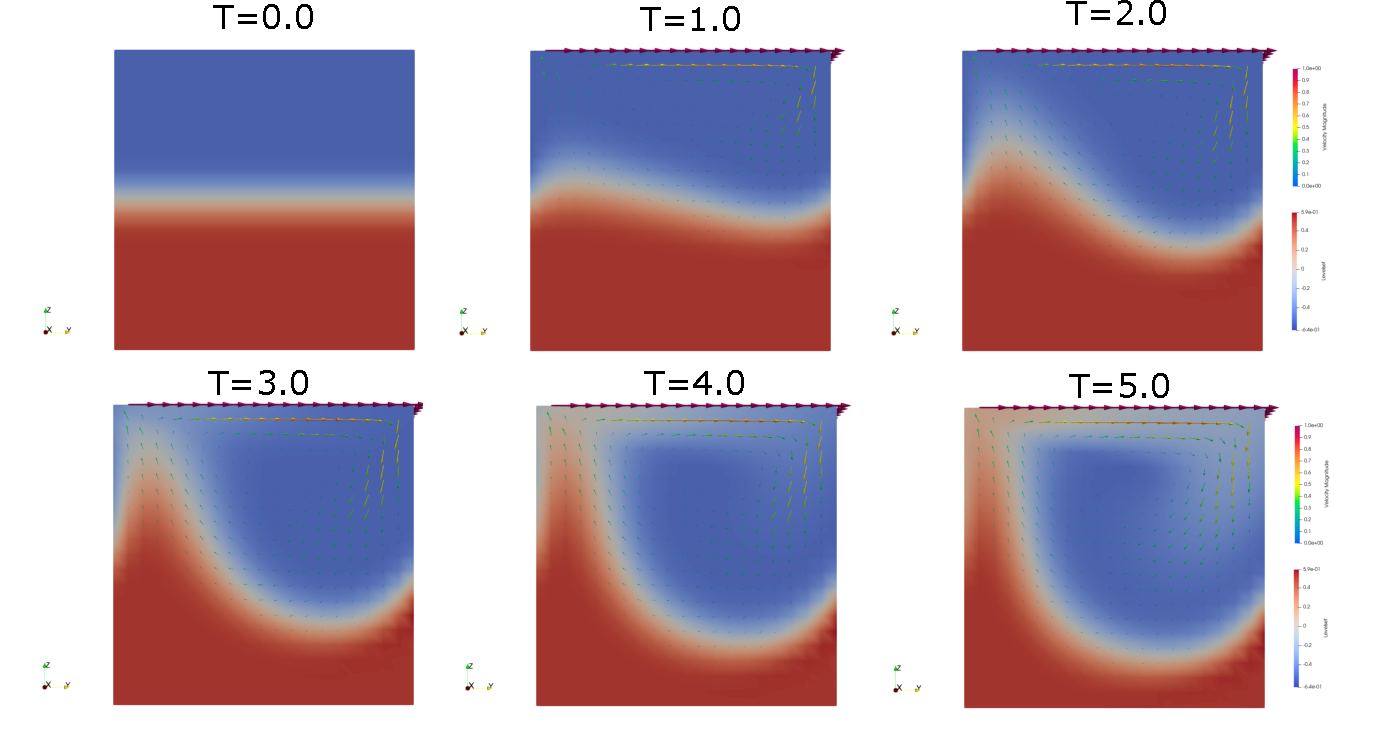
\includegraphics[width=18truecm]{pics/3d-cavity/levelset_velocity.pdf}
	\caption{二層キャビティ流れのレベルセット関数の時間変化}
	\label{fig:3d-bubble-levelset_t0-3}
\end{figure}

\begin{figure}[H]
	\centering
	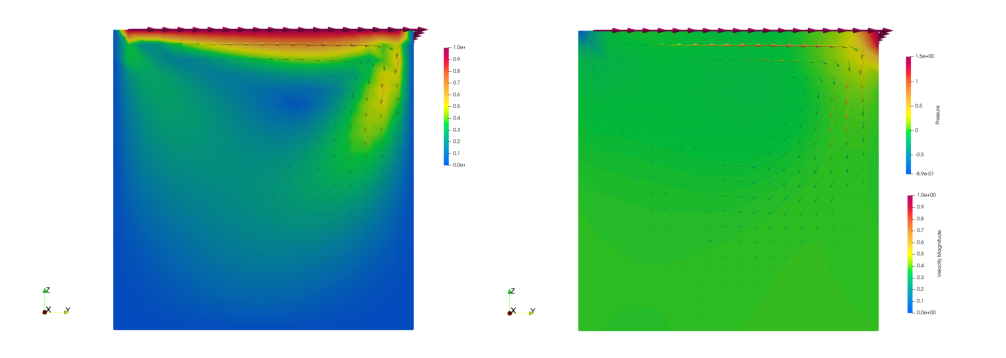
\includegraphics[width=18truecm]{pics/3d-cavity/velocity_pressure.pdf}
	\caption{二層キャビティ流れの速度と圧力分布$(T=30.0)$}
	\label{fig:3d-bubble-levelset_t0-3}
\end{figure}

\begin{figure}[H]
	\centering
	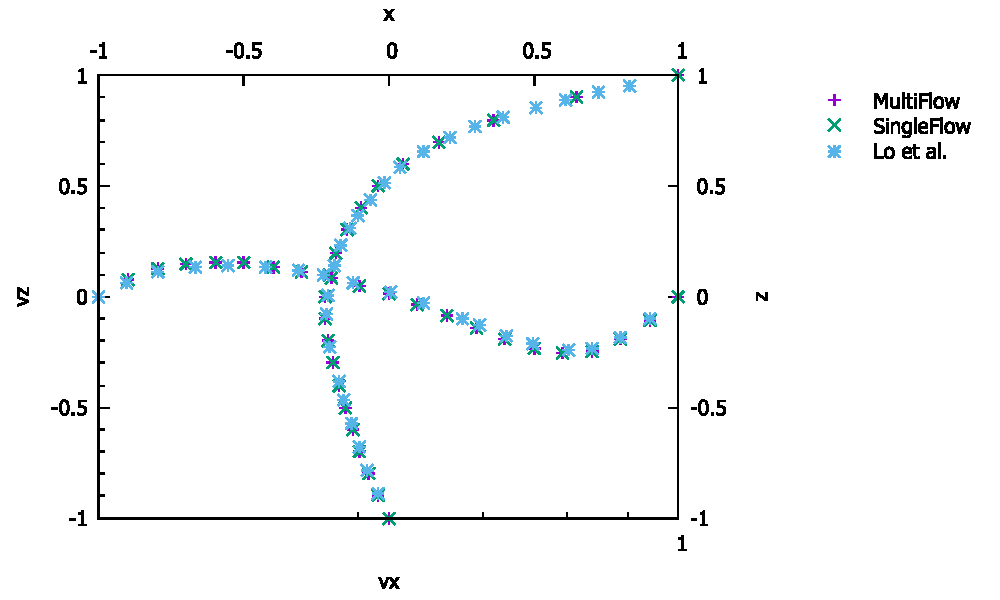
\includegraphics[width=18truecm]{pics/3d-cavity/velocity_graph.pdf}
	\caption{二層キャビティ流れと一層キャビティ流れの速度分布の比較によるプログラム検証$(T=30.0)$}
	\label{fig:3d-cavity_velocity_graph}
\end{figure}

Figure \ref{fig:3d-cavity_velocity_graph}より、単層流の場合と二層流の場合で速度分布が一致しており、参考文献\cite{Lo2005}との結果もよく一致していることがわかるため、プログラムの妥当性を検証できた。

\newpage
\section{3次元のダムブレイク問題}
二層流のベンチマーク問題として3次元のダムブレイク問題を解析した。

\subsection{解析条件}

Table \ref{table:dambreak-material-property}に二つの流体の物性値を示す。
\renewcommand{\arraystretch}{1}
\begin{table}[H]
	\centering
	\caption{物性値}
	\begin{tabular}{ccccccc}
		\hline
		Test case & $\rho_1$ & $\rho_2$ & $\mu_1$ & $\mu_2$ & $\mathrm{g}$ \\
		\hline 
		Case$1$ & $1000$ & $1$   & $1\times10^{-3}$ & $1\times10^{-5}$ & $9.81$ \\
		Case$2$ & $1000$ & $10$  & $1\times10^{-3}$ & $1\times10^{-4}$ & $9.81$ \\
		\hline         
	\end{tabular}
	\label{table:dambreak-material-property}
\end{table}
\renewcommand{\arraystretch}{1.0}

Table \ref{table:dambreak-parameter}に解析パラメータを示す。
\renewcommand{\arraystretch}{1}
\begin{table}[H]
	\centering
	\caption{解析パラメータ}
	\begin{tabular}{cccc}
		\hline
		Test case & $\Delta t$ & メッシュ幅$dx$ & ヘビサイド関数パラメータ$D$\\
		\hline 
		Case$1$ & $0.0001$ & $0.05$ & $0.05$\\
		Case$2$ & $0.0001$ & $0.05$ & $0.15$\\
		\hline         
	\end{tabular}
	\label{table:dambreak-parameter}
\end{table}
\renewcommand{\arraystretch}{1.0}

Figure \ref{fig:3d-dambreak-mesh}に解析用のメッシュを示す。メッシュは六面体$1$次要素である。
\begin{figure}[H]
	\centering
	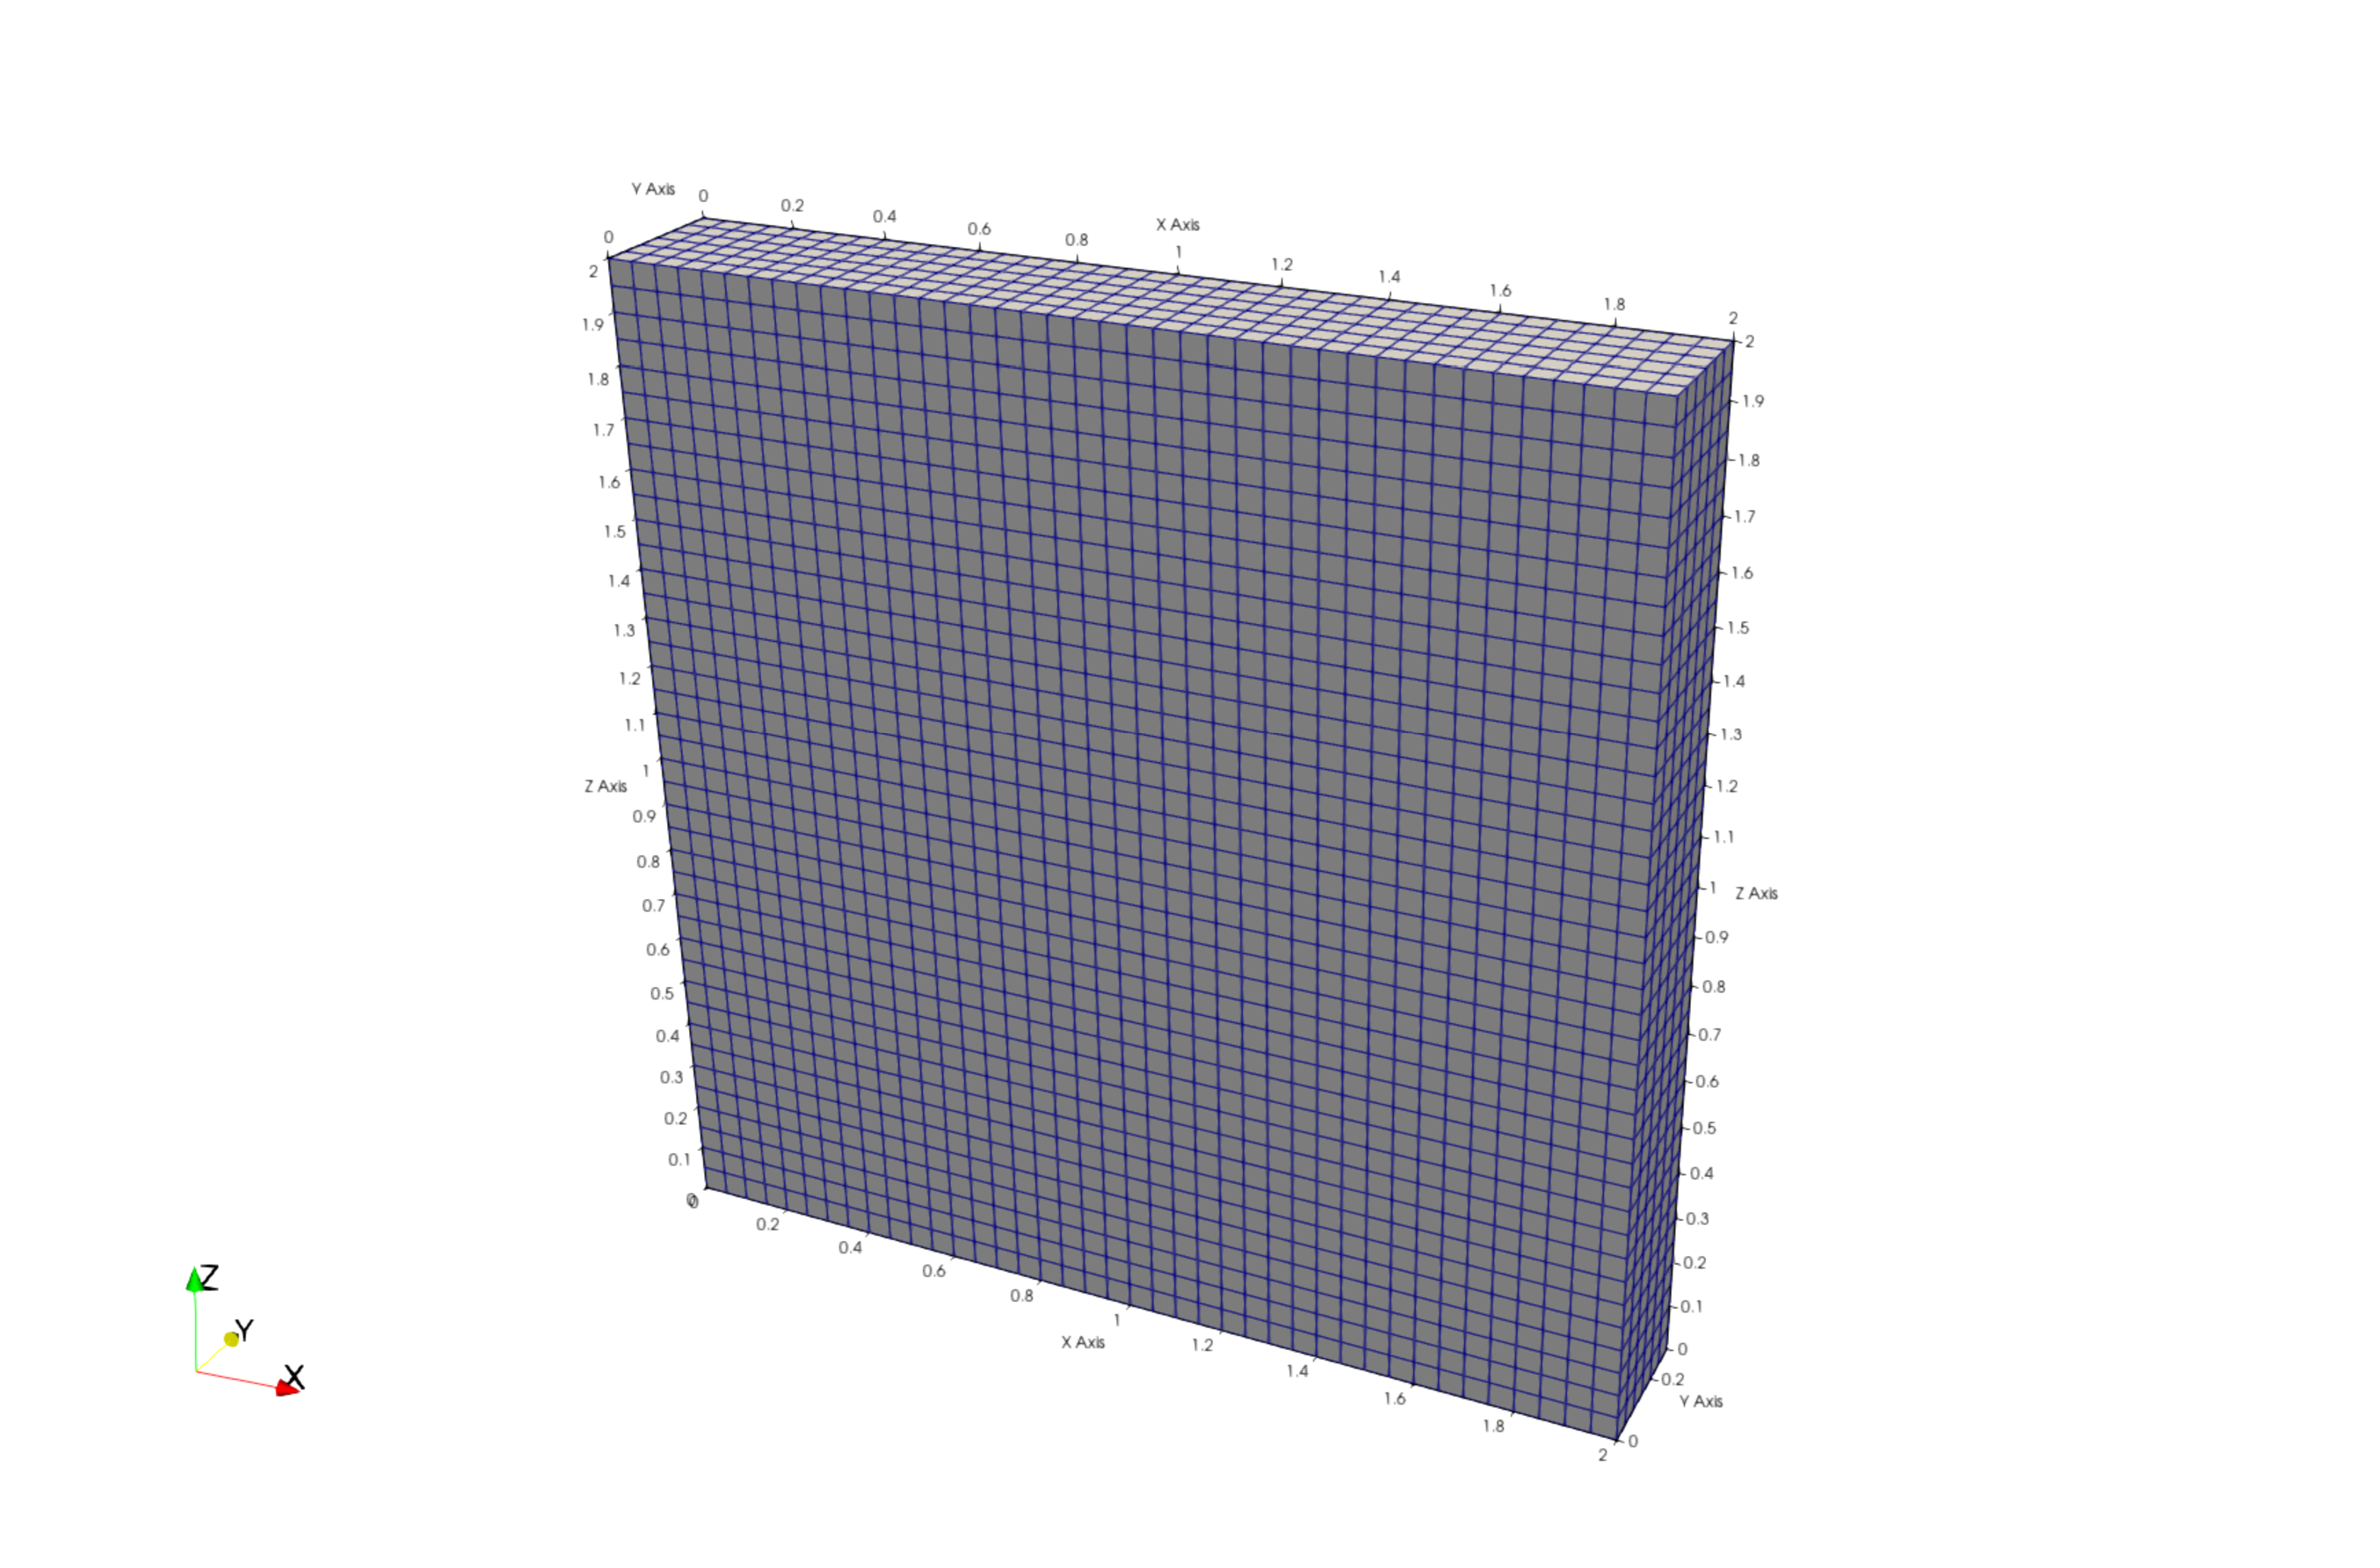
\includegraphics[width=18truecm]{pics/3d-dambreak/mesh.pdf}
	\caption{ダムブレイクの計算メッシュ}
	\label{fig:3d-dambreak-mesh}
\end{figure}

\begin{figure}[H]
	\centering
	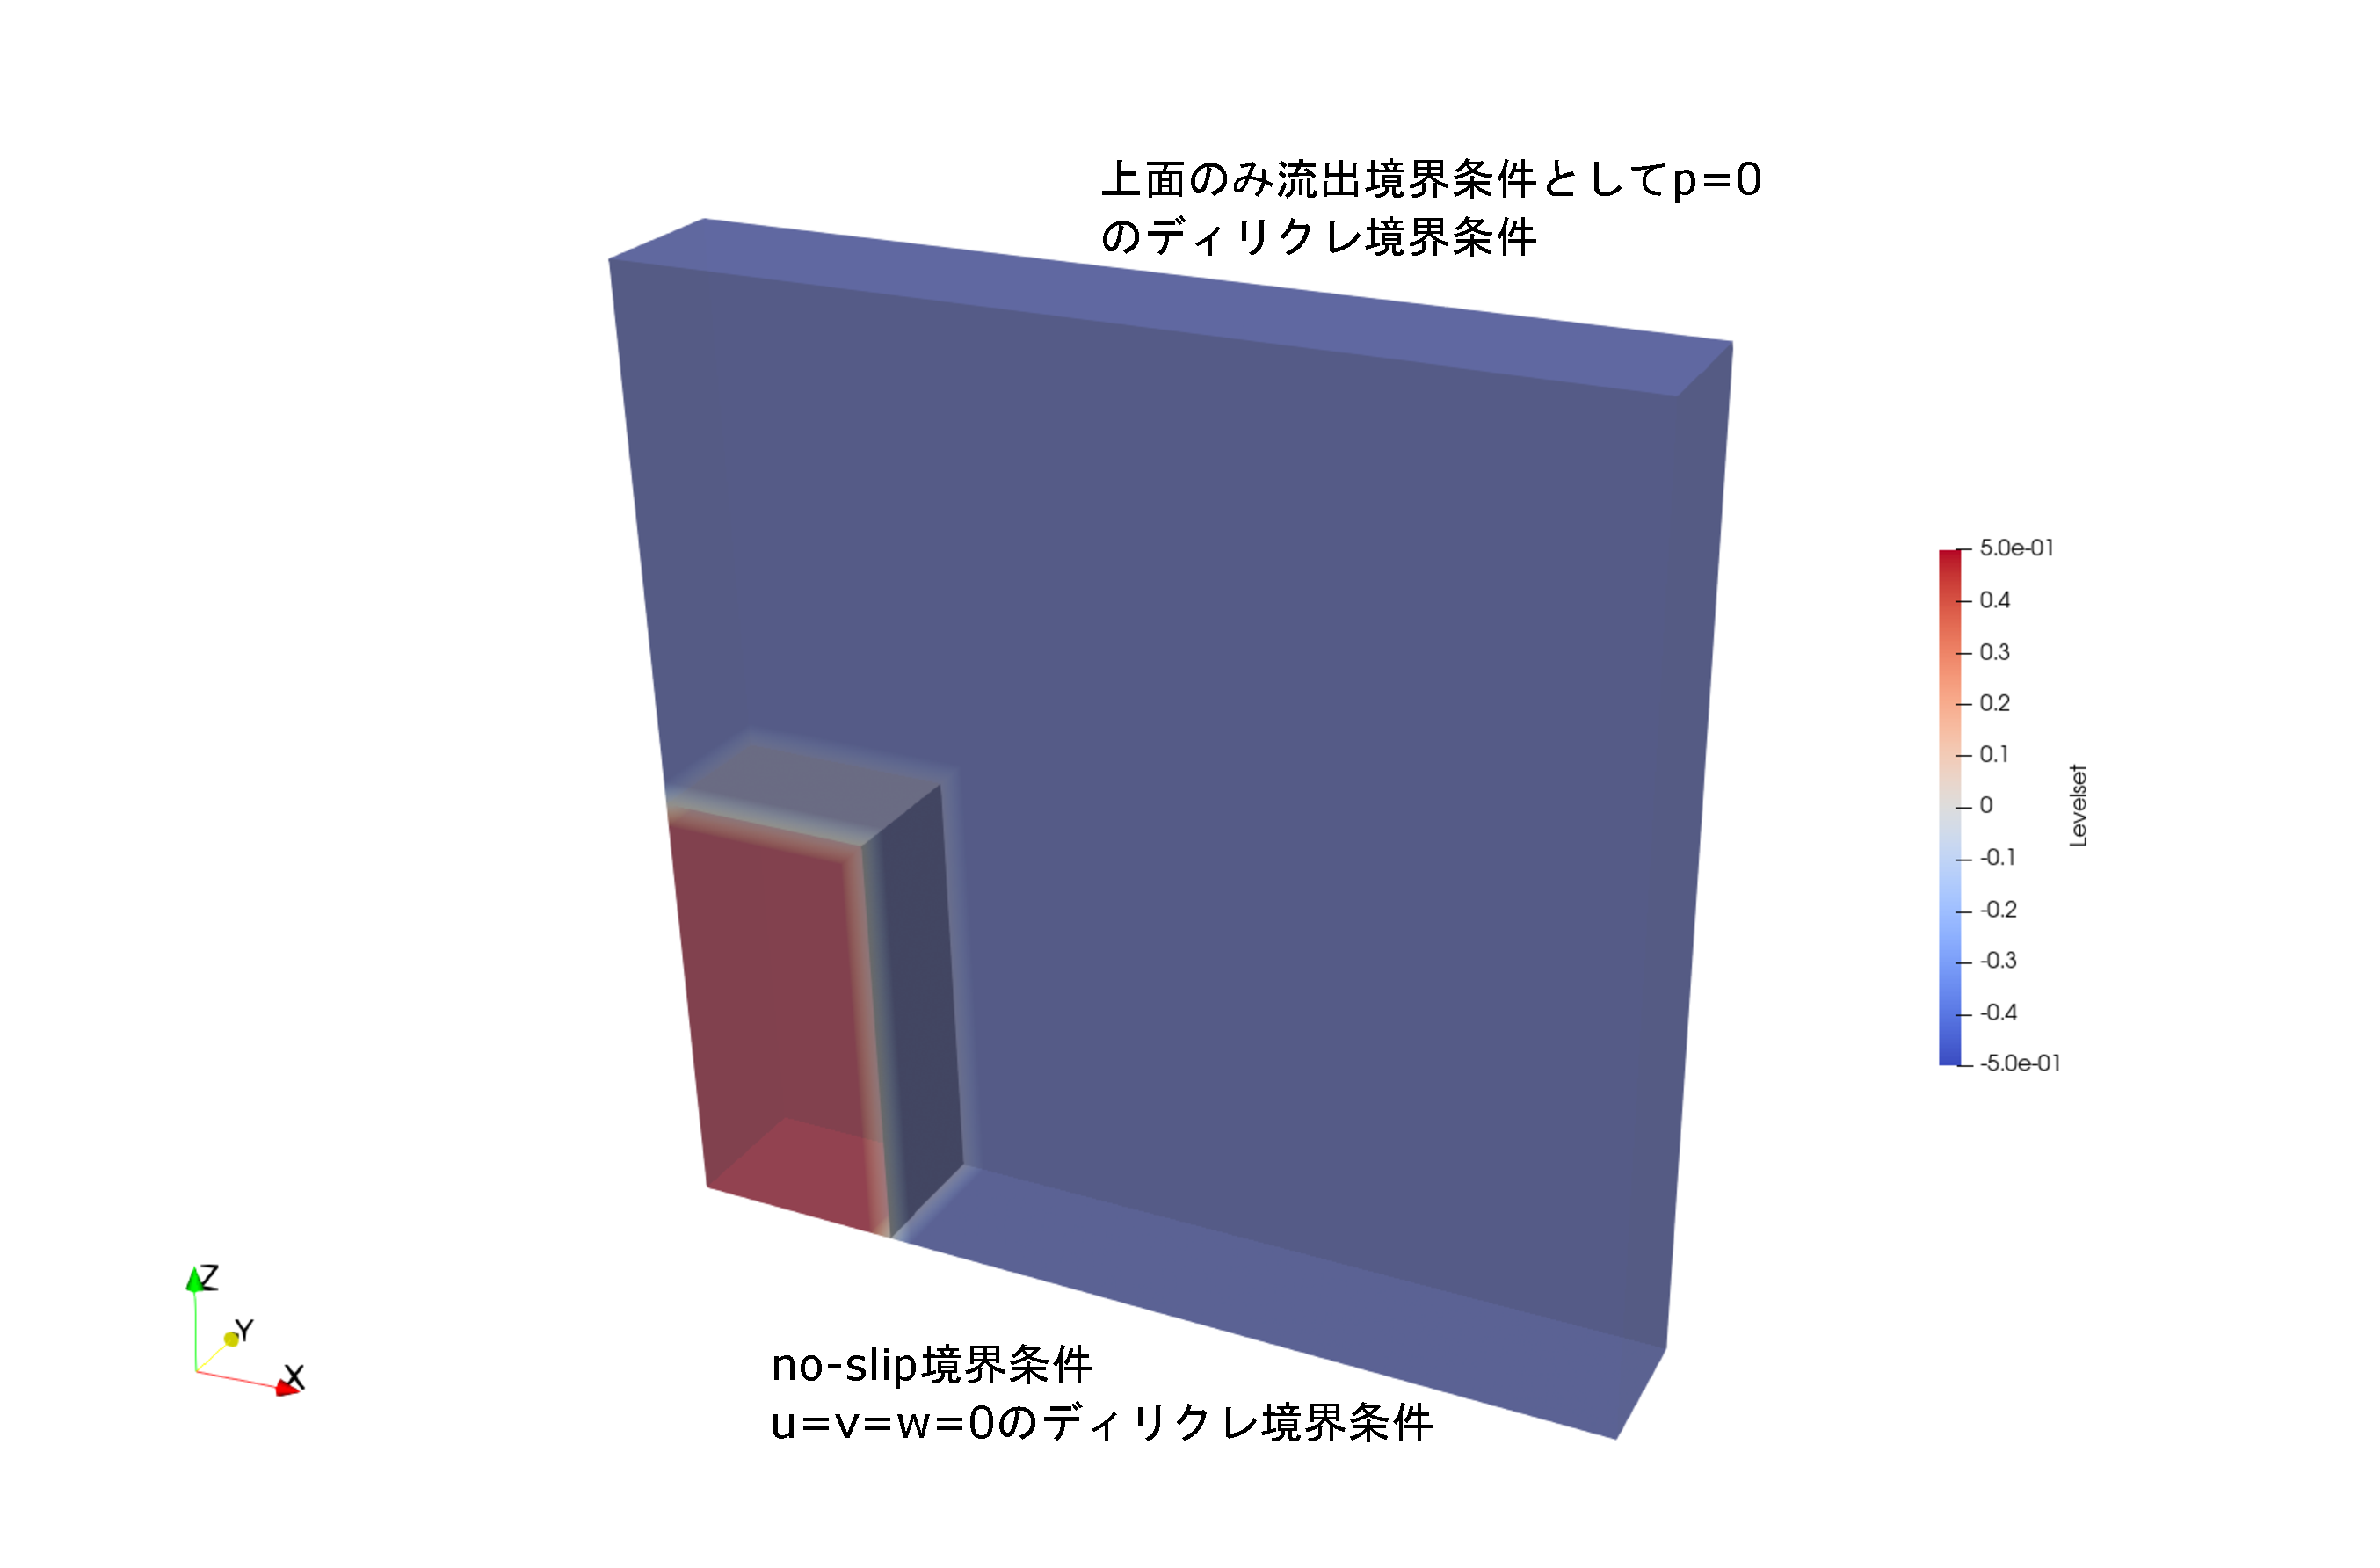
\includegraphics[width=18truecm]{pics/3d-dambreak/levelset_init.pdf}
	\caption{ダムブレイクの初期のレベルセット関数と境界条件}
	\label{fig:3d-dambreak-mesh}
\end{figure}

\subsection{解析結果}

物性値Case$1$の水と空気の物性値のオーダーでは計算が発散してしまう。解析パラメータ$1$, $2$でも同様に発散する。
物性値Case$2$の水と空気(の密度と粘性係数が10倍)の物性値のオーダーでは、解析パラメータ$1$では発散し、$2$でヘビサイド関数の$D$を大きく取ることで安定化した。

\begin{figure}[H]
	\centering
	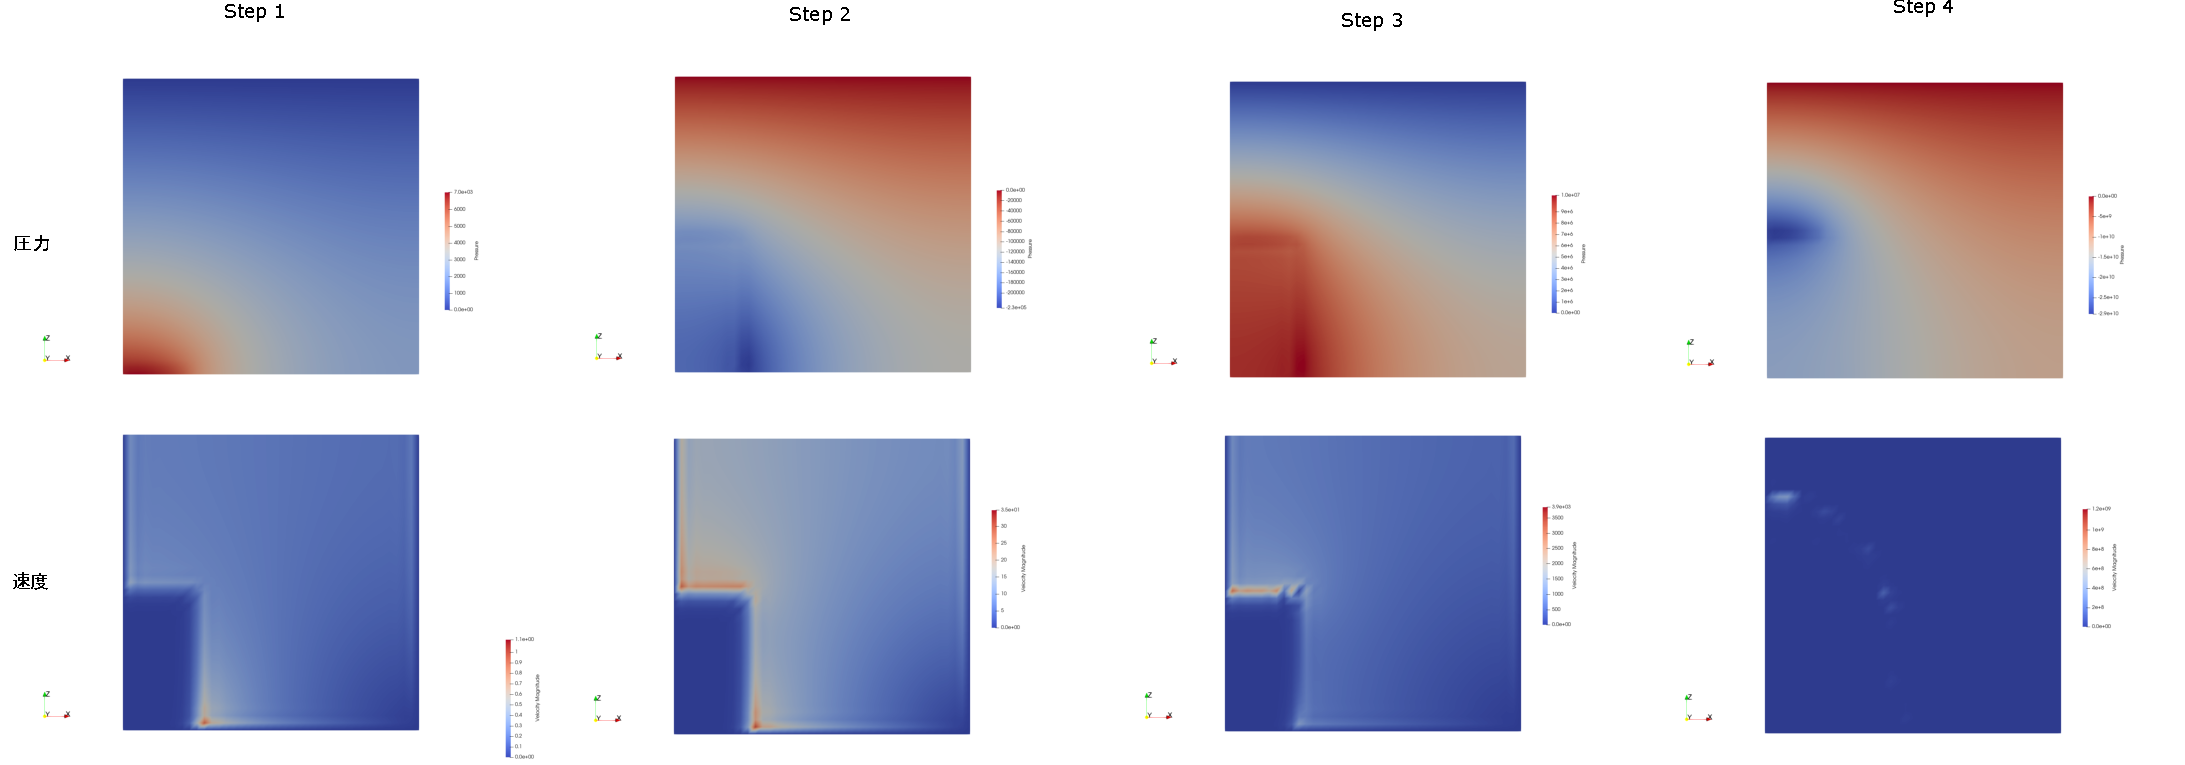
\includegraphics[width=18truecm]{pics/3d-dambreak/diverge_water_air.pdf}
	\caption{ダムブレイク問題のCase1の計算結果における速度と圧力分布($y=0.4$における断面)。物性値がCase1の差が大きい場合の初期の発散する様子と圧力が振動していることがわかる。}
	\label{fig:3d-dambreak-diverge}
\end{figure}

\begin{figure}[H]
	\centering
	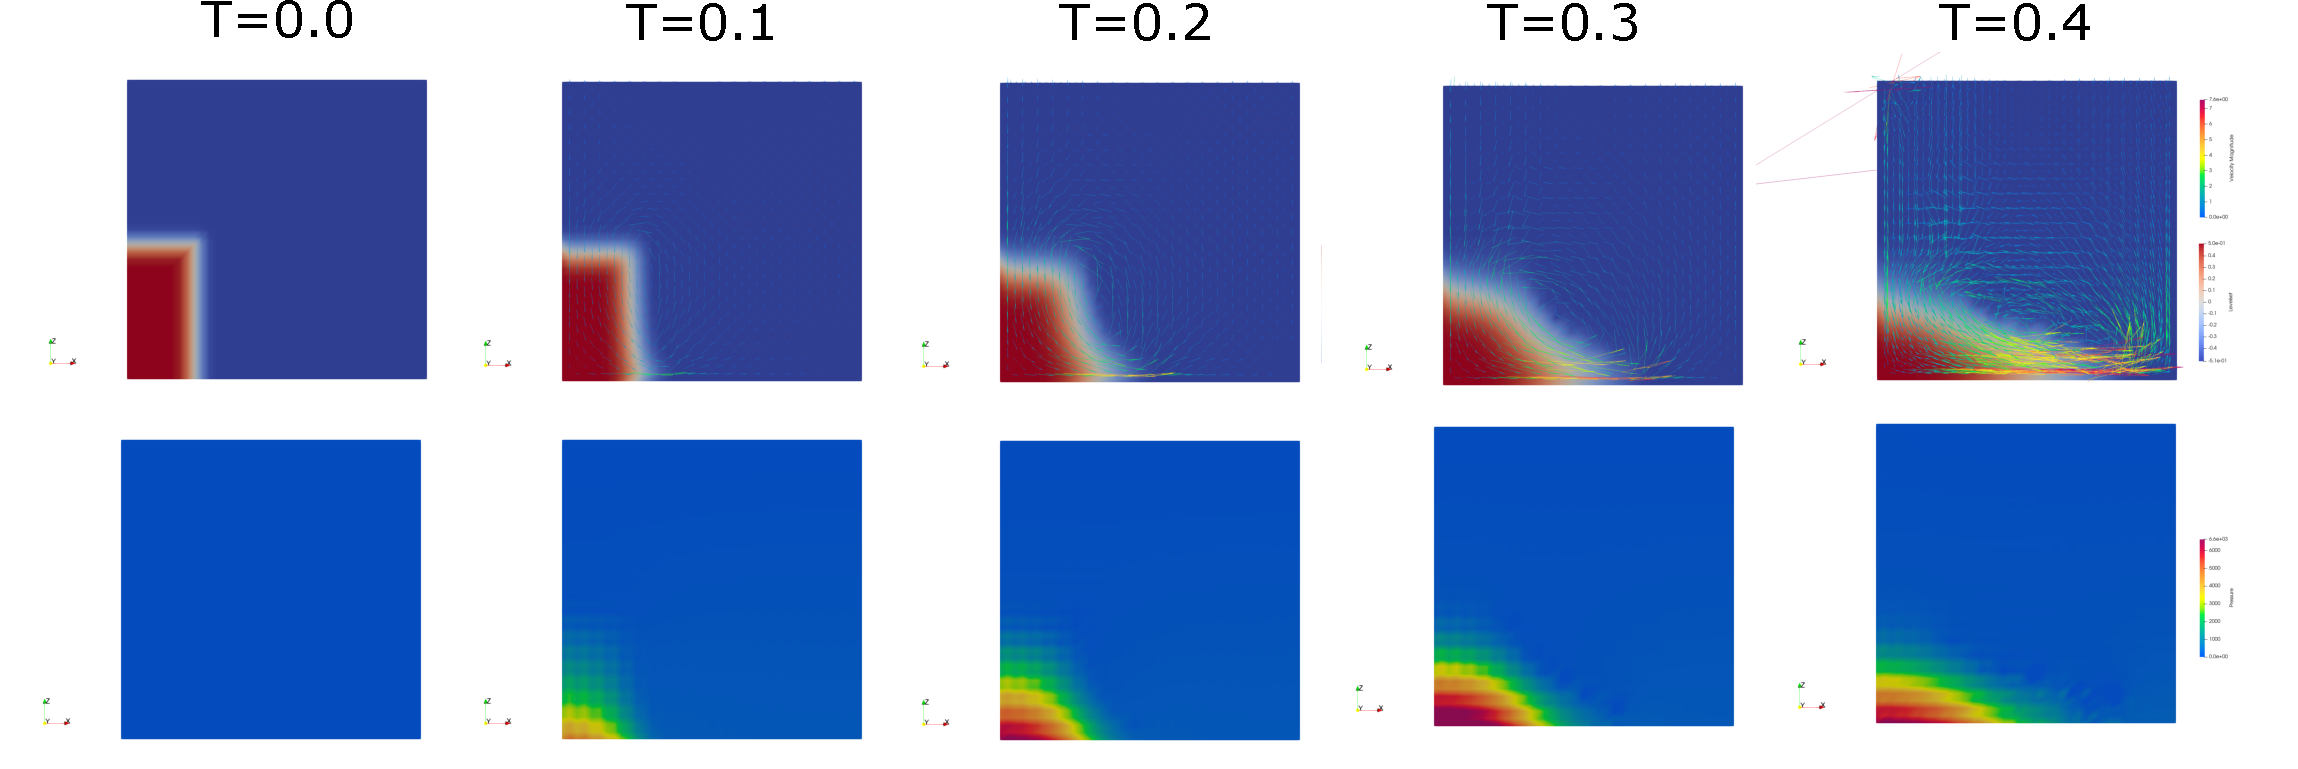
\includegraphics[width=18truecm]{pics/3d-dambreak/levelset_velocity.pdf}
	\caption{ダムブレイク問題のCase2の計算結果における速度と圧力分布($y=0.4$における断面)。Case2の物性値の差が小さい場合ではヘビサイド関数Dの値を大きくすることで安定に計算可能となった。}
	\label{fig:3d-dambreak-diverge}
\end{figure}

\subsection{並列解析結果}
ここでは、3.5項で示した並列化解析実行手順に従い並列数を4として並列解析をした結果を示す。
Figure \ref{fig:3d-dambreak-parallel-partition}に領域分割したメッシュを示す。

\begin{figure}[H]
	\centering
	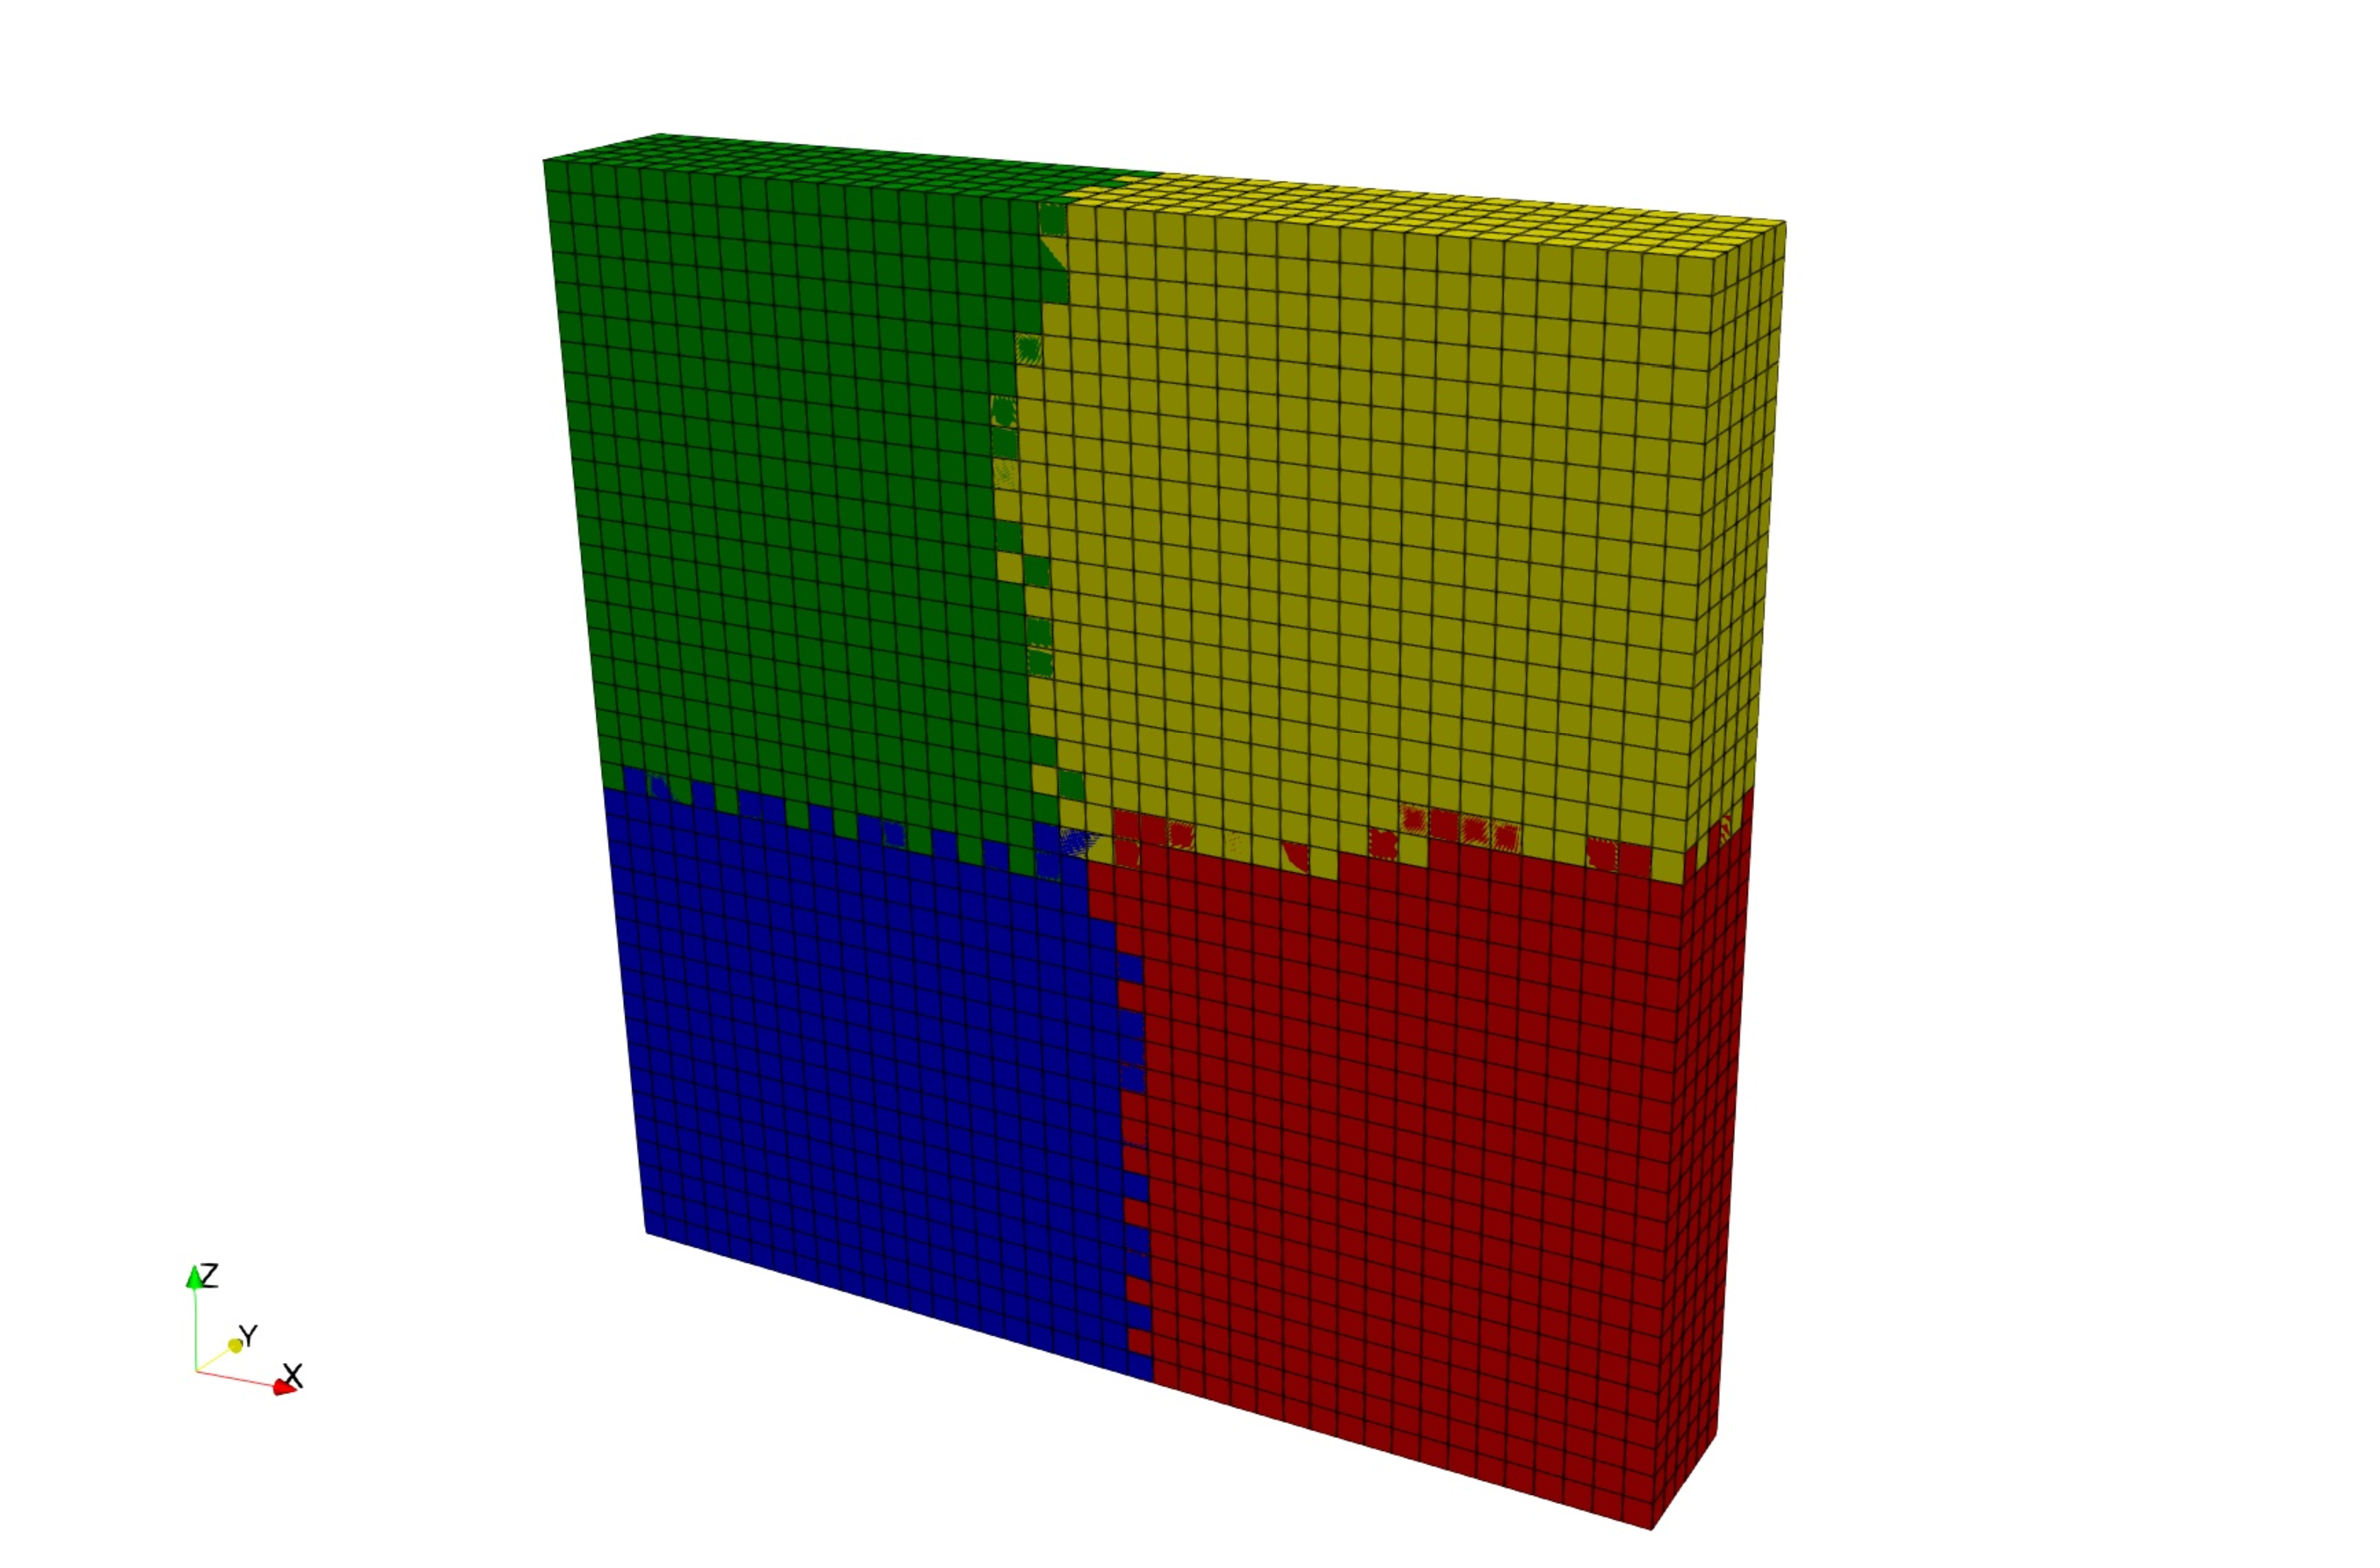
\includegraphics[width=18truecm]{pics/3d-dambreak-parallel/partition4.pdf}
	\caption{並列数4の場合の領域分割の図}
	\label{fig:3d-dambreak-parallel-partition}
\end{figure}

Figure \ref{fig:3d-dambreak-parallel-result}に速度分布、圧力分布、レベルセット関数の結果を示す。
並列化なしの場合と同様の結果が得られており、並列化解析が問題なくできていることが確認できた。

\begin{figure}[H]
	\centering
	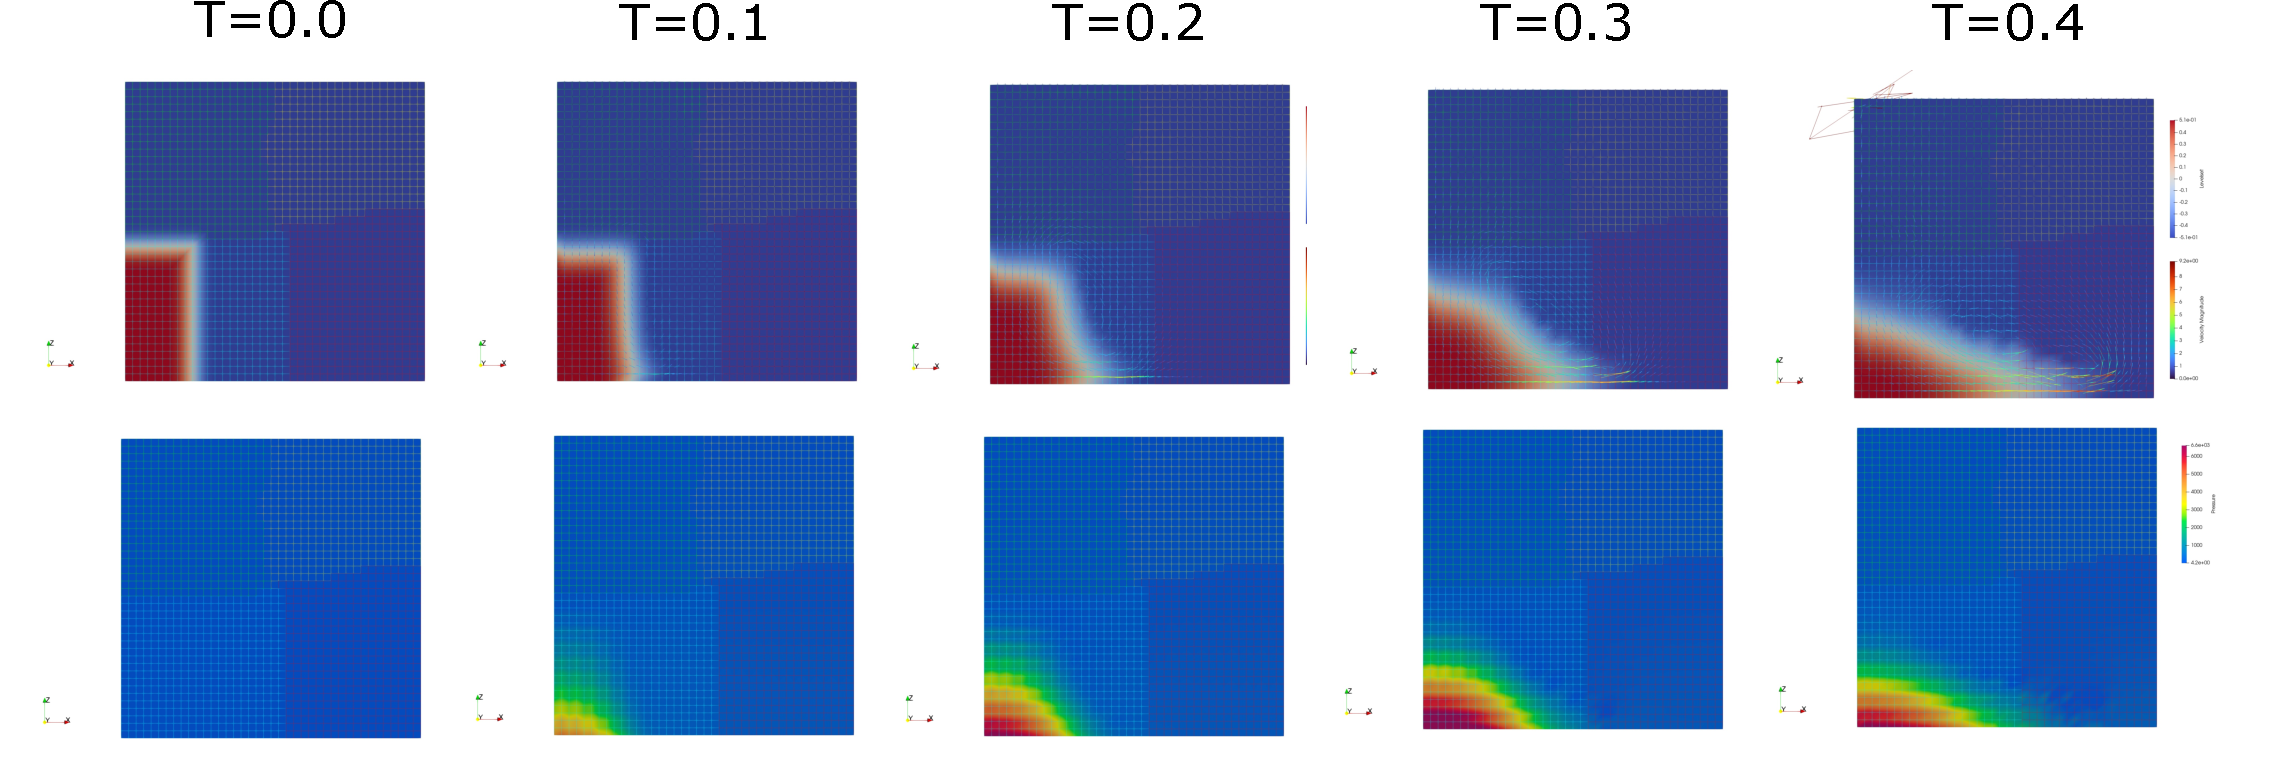
\includegraphics[width=18truecm]{pics/3d-dambreak-parallel/result-partition4.pdf}
	\caption{ダムブレイク問題のCase2の並列化解析による計算結果($y=0.4$における断面)。網目の色の違いで領域分割されている領域を可視化した。}
	\label{fig:3d-dambreak-parallel-result}
\end{figure}

\newpage
\section{3次元の気泡上昇問題}
3次元の解析の定量的な精度検証として、気泡上昇問題を解析し、参考文献の結果と比較した。
\subsection{解析条件}
Table \ref{table:3d-bubble-material-property}に物性値を示す。

\renewcommand{\arraystretch}{1}
\begin{table}[H]
	\centering
	\caption{解析パラメータ}
	\begin{tabular}{ccccccc}
		\hline
		Test case & $\rho_1$ & $\rho_2$ & $\mu_1$ & $\mu_2$ & $\mathrm{g}$ & $\sigma$\\
		\hline 
		Case$1$ & $1000$ & $100$ & $10$ & $1$   & $0.98$ & $24.5$ \\
		Case$2$ & $1000$ & $1$   & $10$ & $0.1$ & $0.98$ & $1.96$ \\
		\hline         
	\end{tabular}
	\label{table:3d-bubble-material-property}
\end{table}
\renewcommand{\arraystretch}{1.0}

Table \ref{table:3d-bubble-parameter}に解析パラメータを示す。
\renewcommand{\arraystretch}{1}
\begin{table}[H]
	\centering
	\caption{解析パラメータ}
	\begin{tabular}{ccc}
		\hline
		Test case & メッシュ幅$dx$ & ヘビサイド関数パラメータ$D$\\
		\hline 
		Case$1$ & $0.05$ & $0.05$\\
		\hline         
	\end{tabular}
	\label{table:3d-bubble-parameter}
\end{table}
\renewcommand{\arraystretch}{1.0}

\begin{figure}[H]
	\centering
	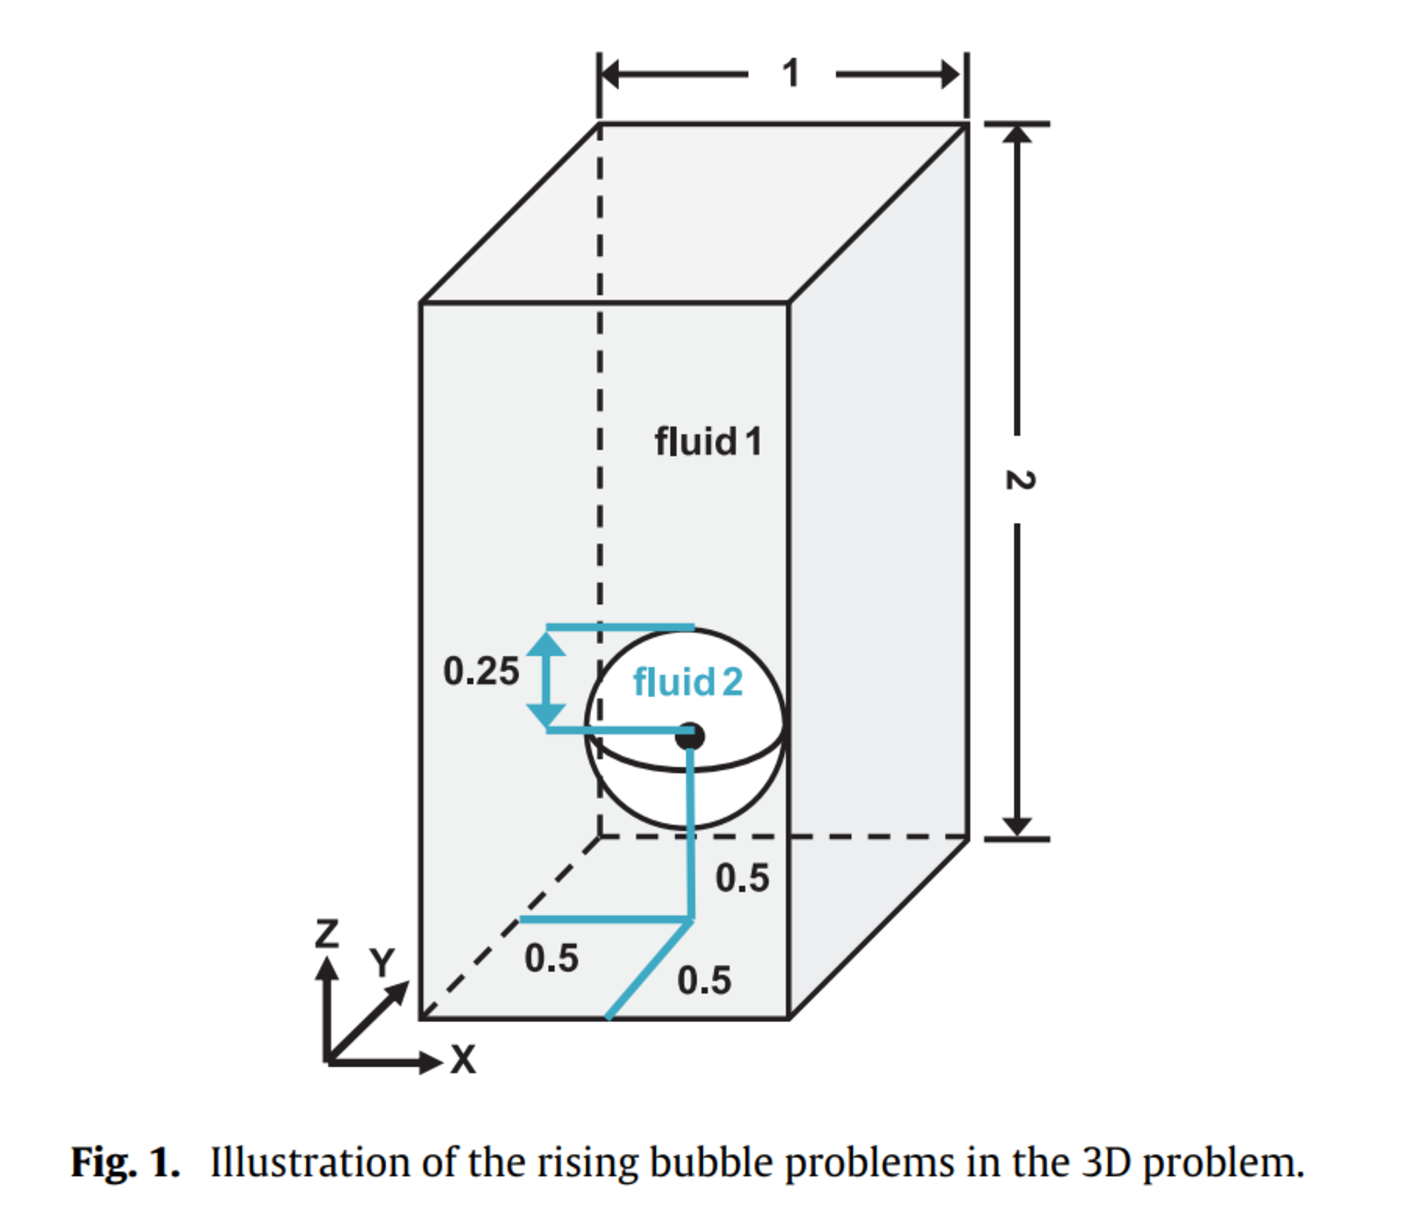
\includegraphics[width=10truecm]{pics/3d-bubble/setting.pdf}
	\caption{解析条件\cite{Safi2017}}
	\label{fig:3d-bubble-setting}
\end{figure}

Figure \ref{fig:3d-bubble-mesh}に解析用のメッシュを示す。メッシュは四面体$1$次要素である。

\begin{figure}[H]
	\centering
	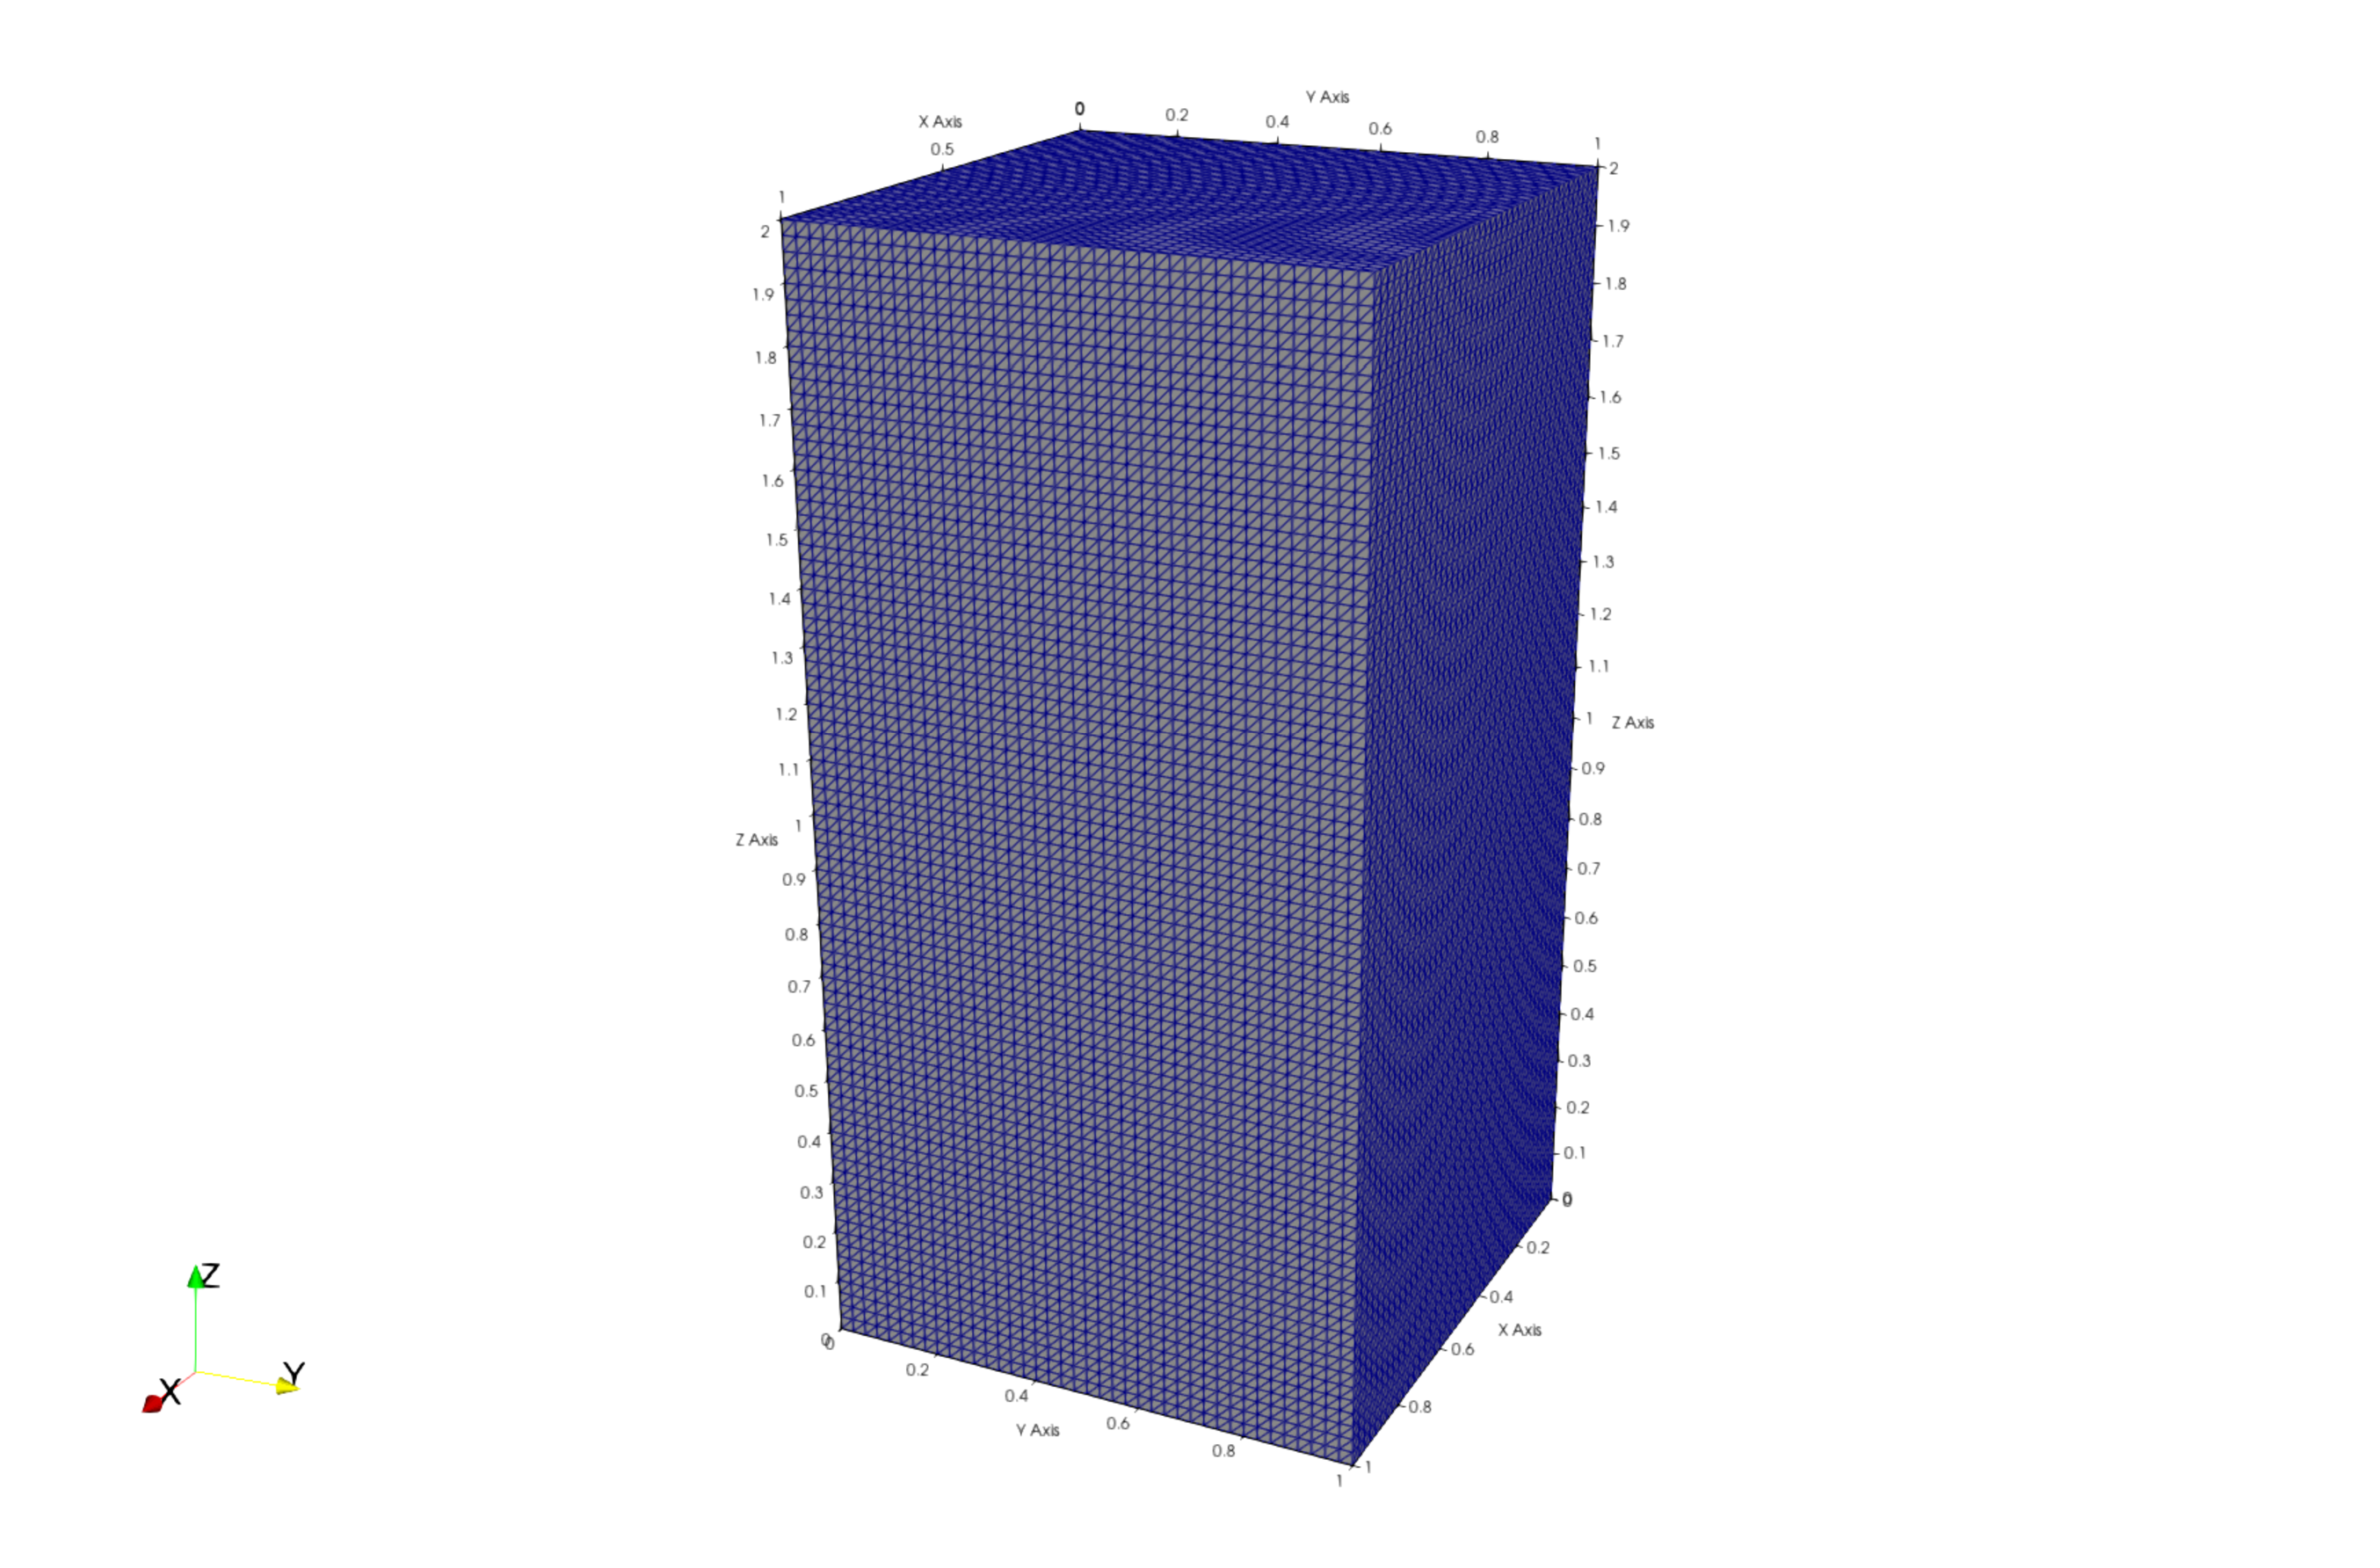
\includegraphics[width=10truecm]{pics/3d-bubble/mesh.pdf}
	\caption{3次元気泡上昇流れの計算メッシュ}
	\label{fig:3d-bubble-mesh}
\end{figure}

Figure \ref{fig:3d-bubble-levelset_t0_3d}に初期状態のレベルセット関数を示す。

\begin{figure}[H]
	\centering
	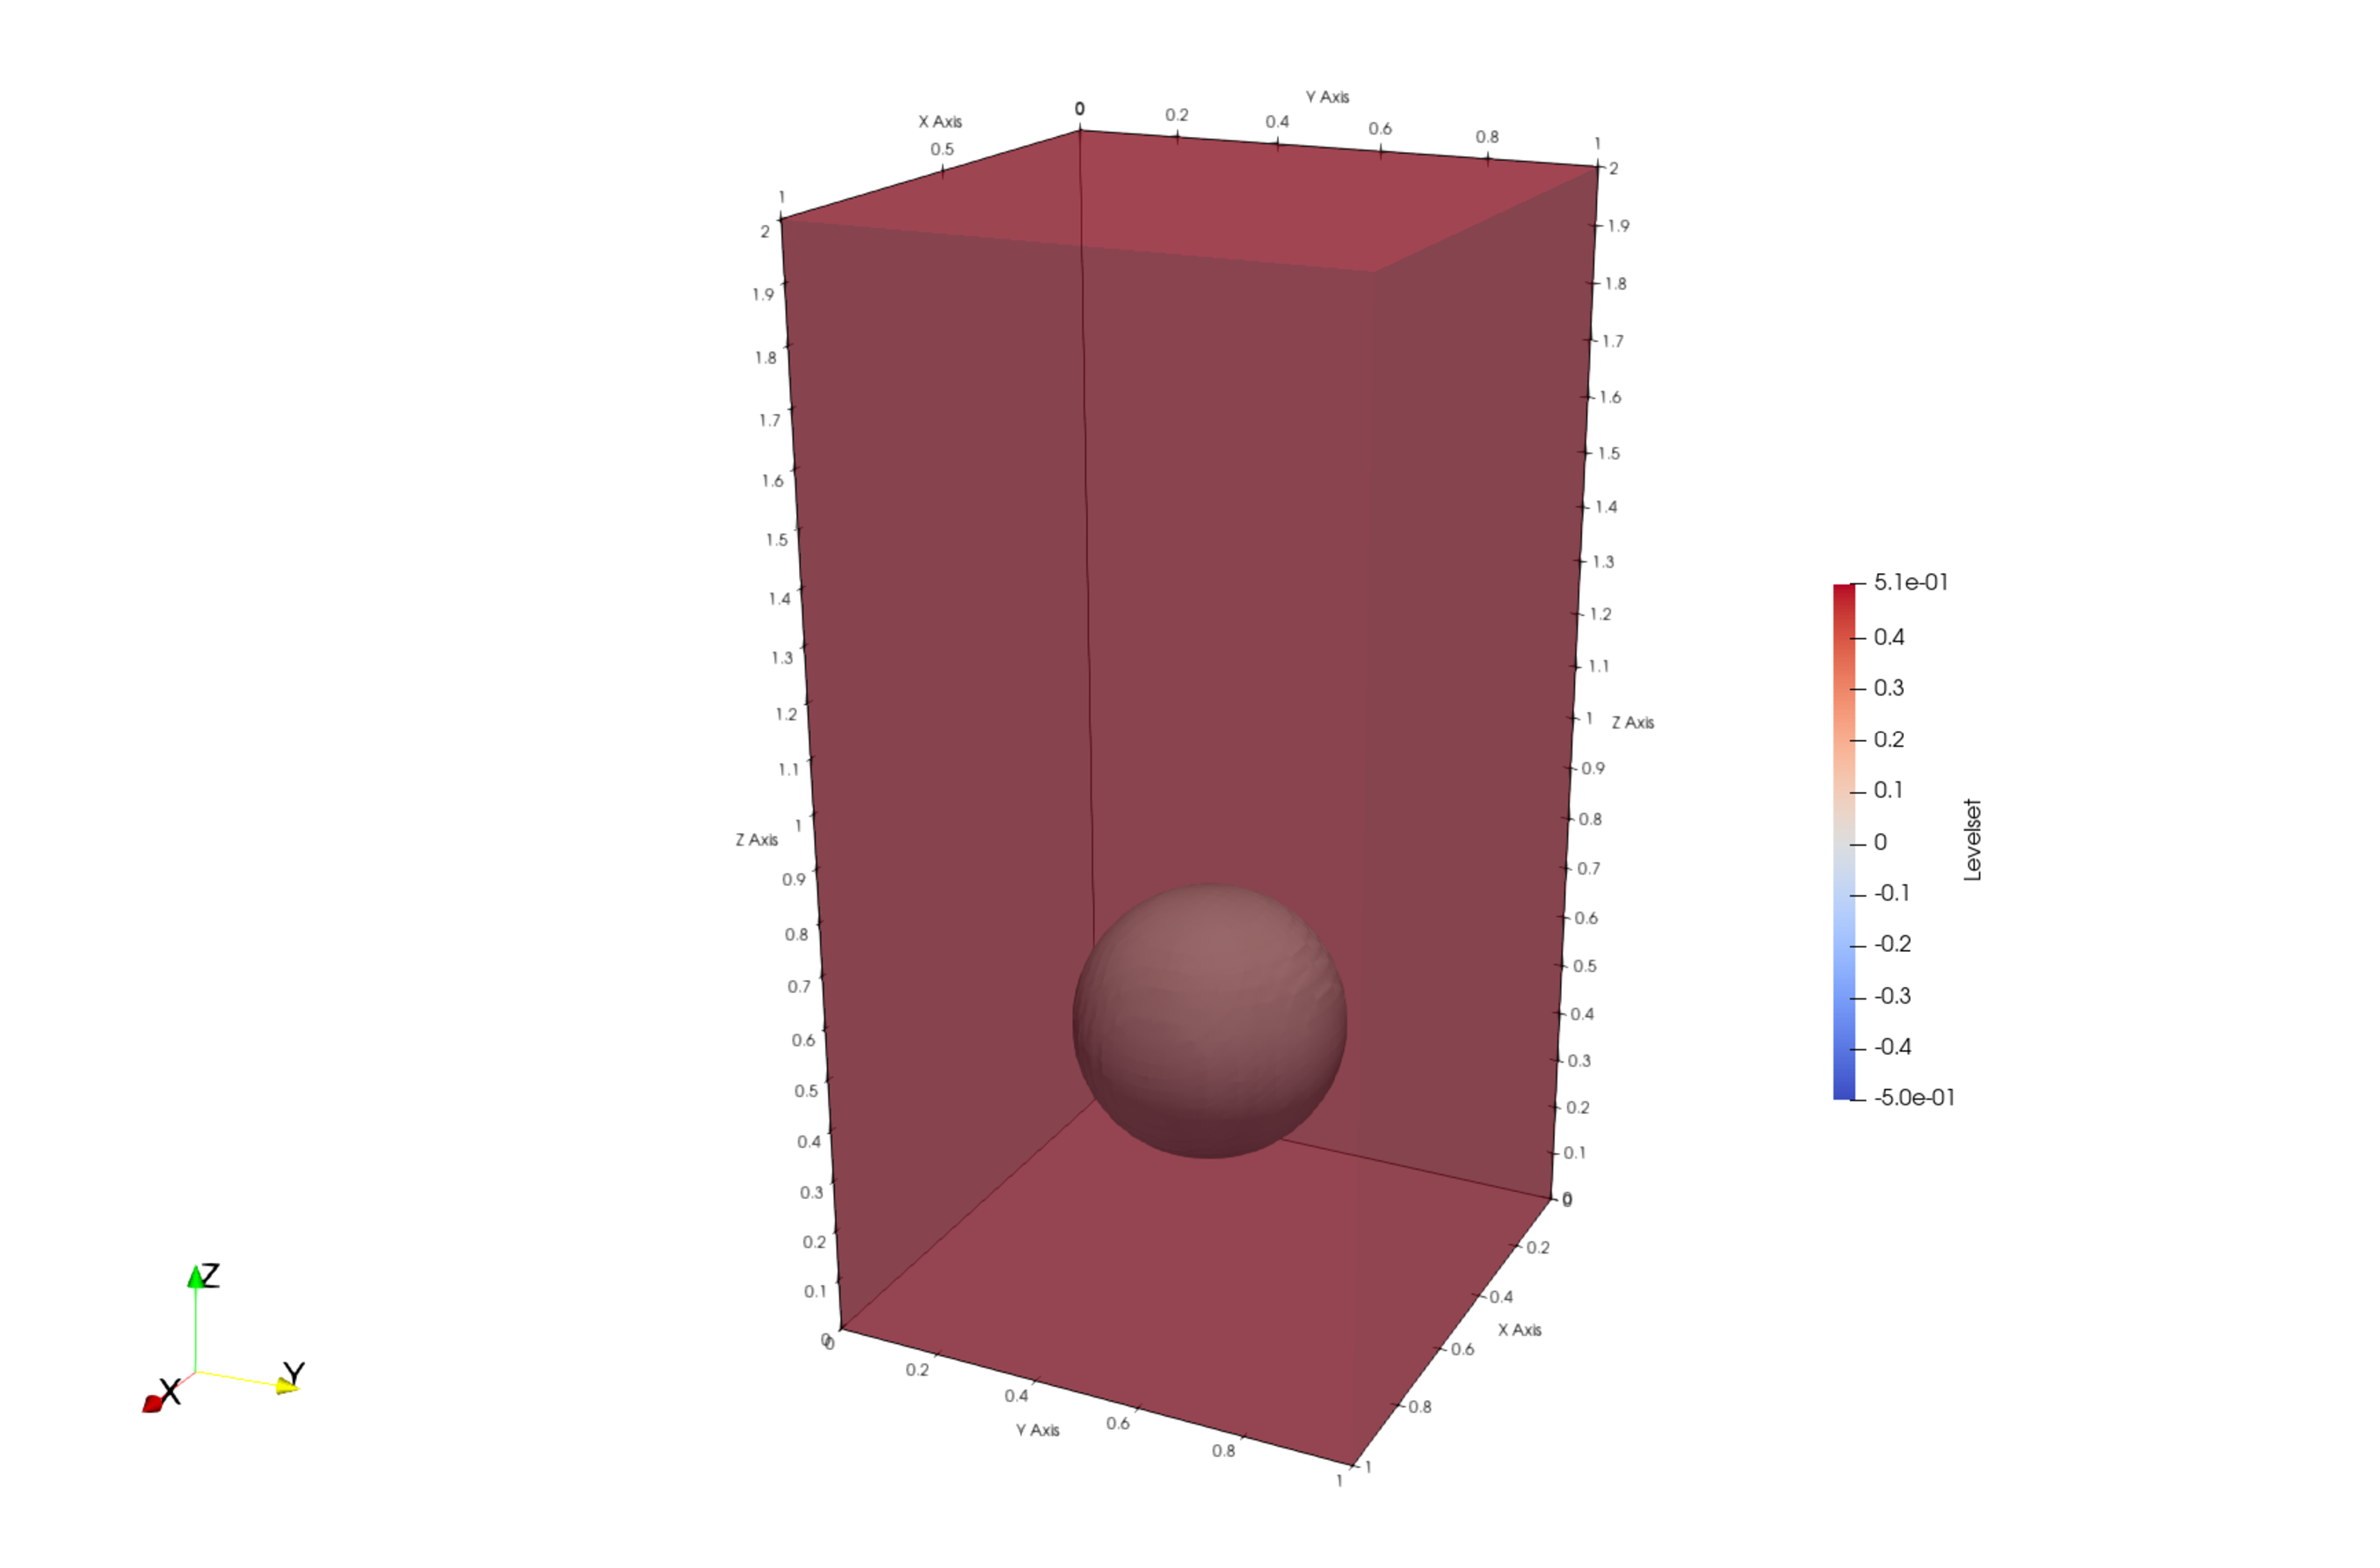
\includegraphics[width=10truecm]{pics/3d-bubble/levelset_t0_3d.pdf}
	\caption{3次元気泡上昇流れの初期状態のレベルセット関数}
	\label{fig:3d-bubble-levelset_t0_3d}
\end{figure}

\subsection{解析結果}

Figure \ref{fig:3d-bubble-result_sigma0}は表面張力を導入する前の表面張力係数$\sigma=0$の場合の結果である。Figure \ref{fig:3d-bubble-result-ref}の参考文献の結果と比較すると形が大きく変形してしまっていることがわかる。
表面張力の有無による差と考え、表面張力のモデルを導入し計算した結果を示す。
Figure \ref{fig:3d-bubble_result_sigma24.5}は文献と同じ表面張力係数$\sigma=24.5$を使用したが、形が崩れていってしまう結果となった。
Figure \ref{fig:3d-bubble_result_sigma9.8}, \ref{fig:3d-bubble_result_sigma4.9}にそれぞれ係数$\sigma$を$9.8, 4.9$と小さくした場合の結果を示す。\ref{fig:3d-bubble_result_sigma4.9}の場合の$T=1.5$と\ref{fig:3d-bubble-result_sigma0}の$T=1.5$を比較すると表面張力によって初期の変形が抑えられており、表面張力の導入の効果は見られるが、参考文献の形状とは差があり、係数を大きくした場合の変形の不安定性を抑えることが課題である。

\begin{figure}[H]
	\centering
	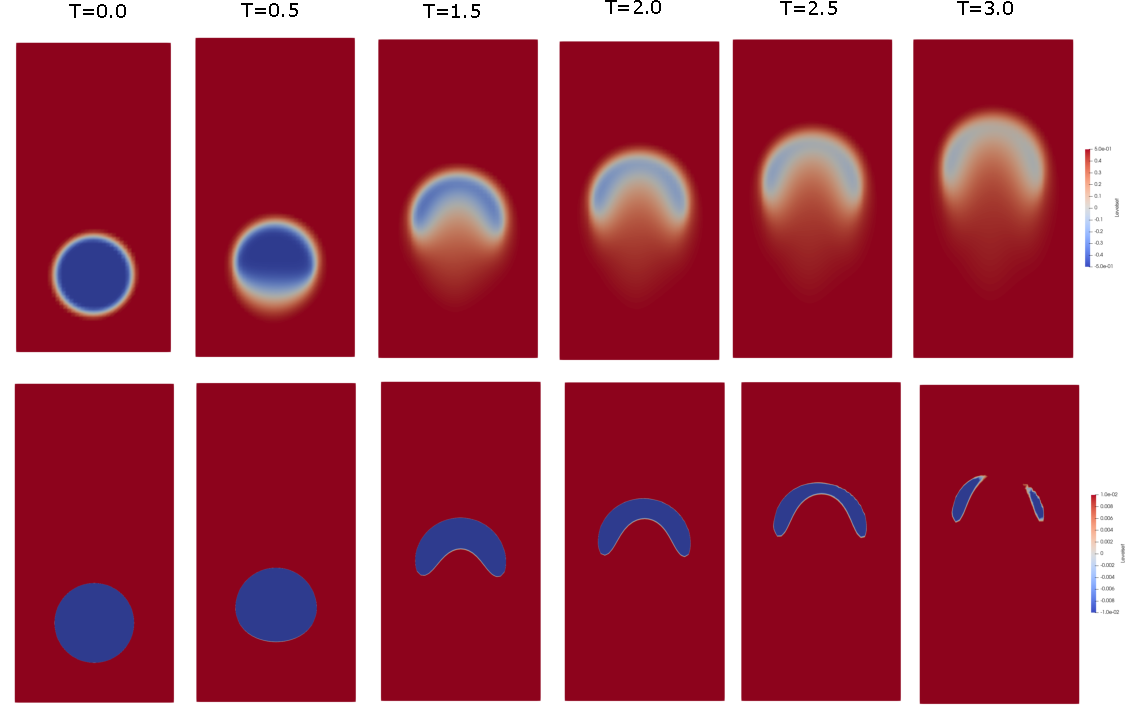
\includegraphics[width=18truecm]{pics/3d-bubble/levelset_t0-3.pdf}
	\caption{3次元気泡上昇流れのレベルセット関数の分布の時間変化($\sigma=0$、表面張力なし)。上はカラーバーの範囲が$-0.5$~$+0.5$、下は$-0.01$~$+0.01$として界面の位置を見やすくしている。}
	\label{fig:3d-bubble-result_sigma0}
\end{figure}

\begin{figure}[H]
	\centering
	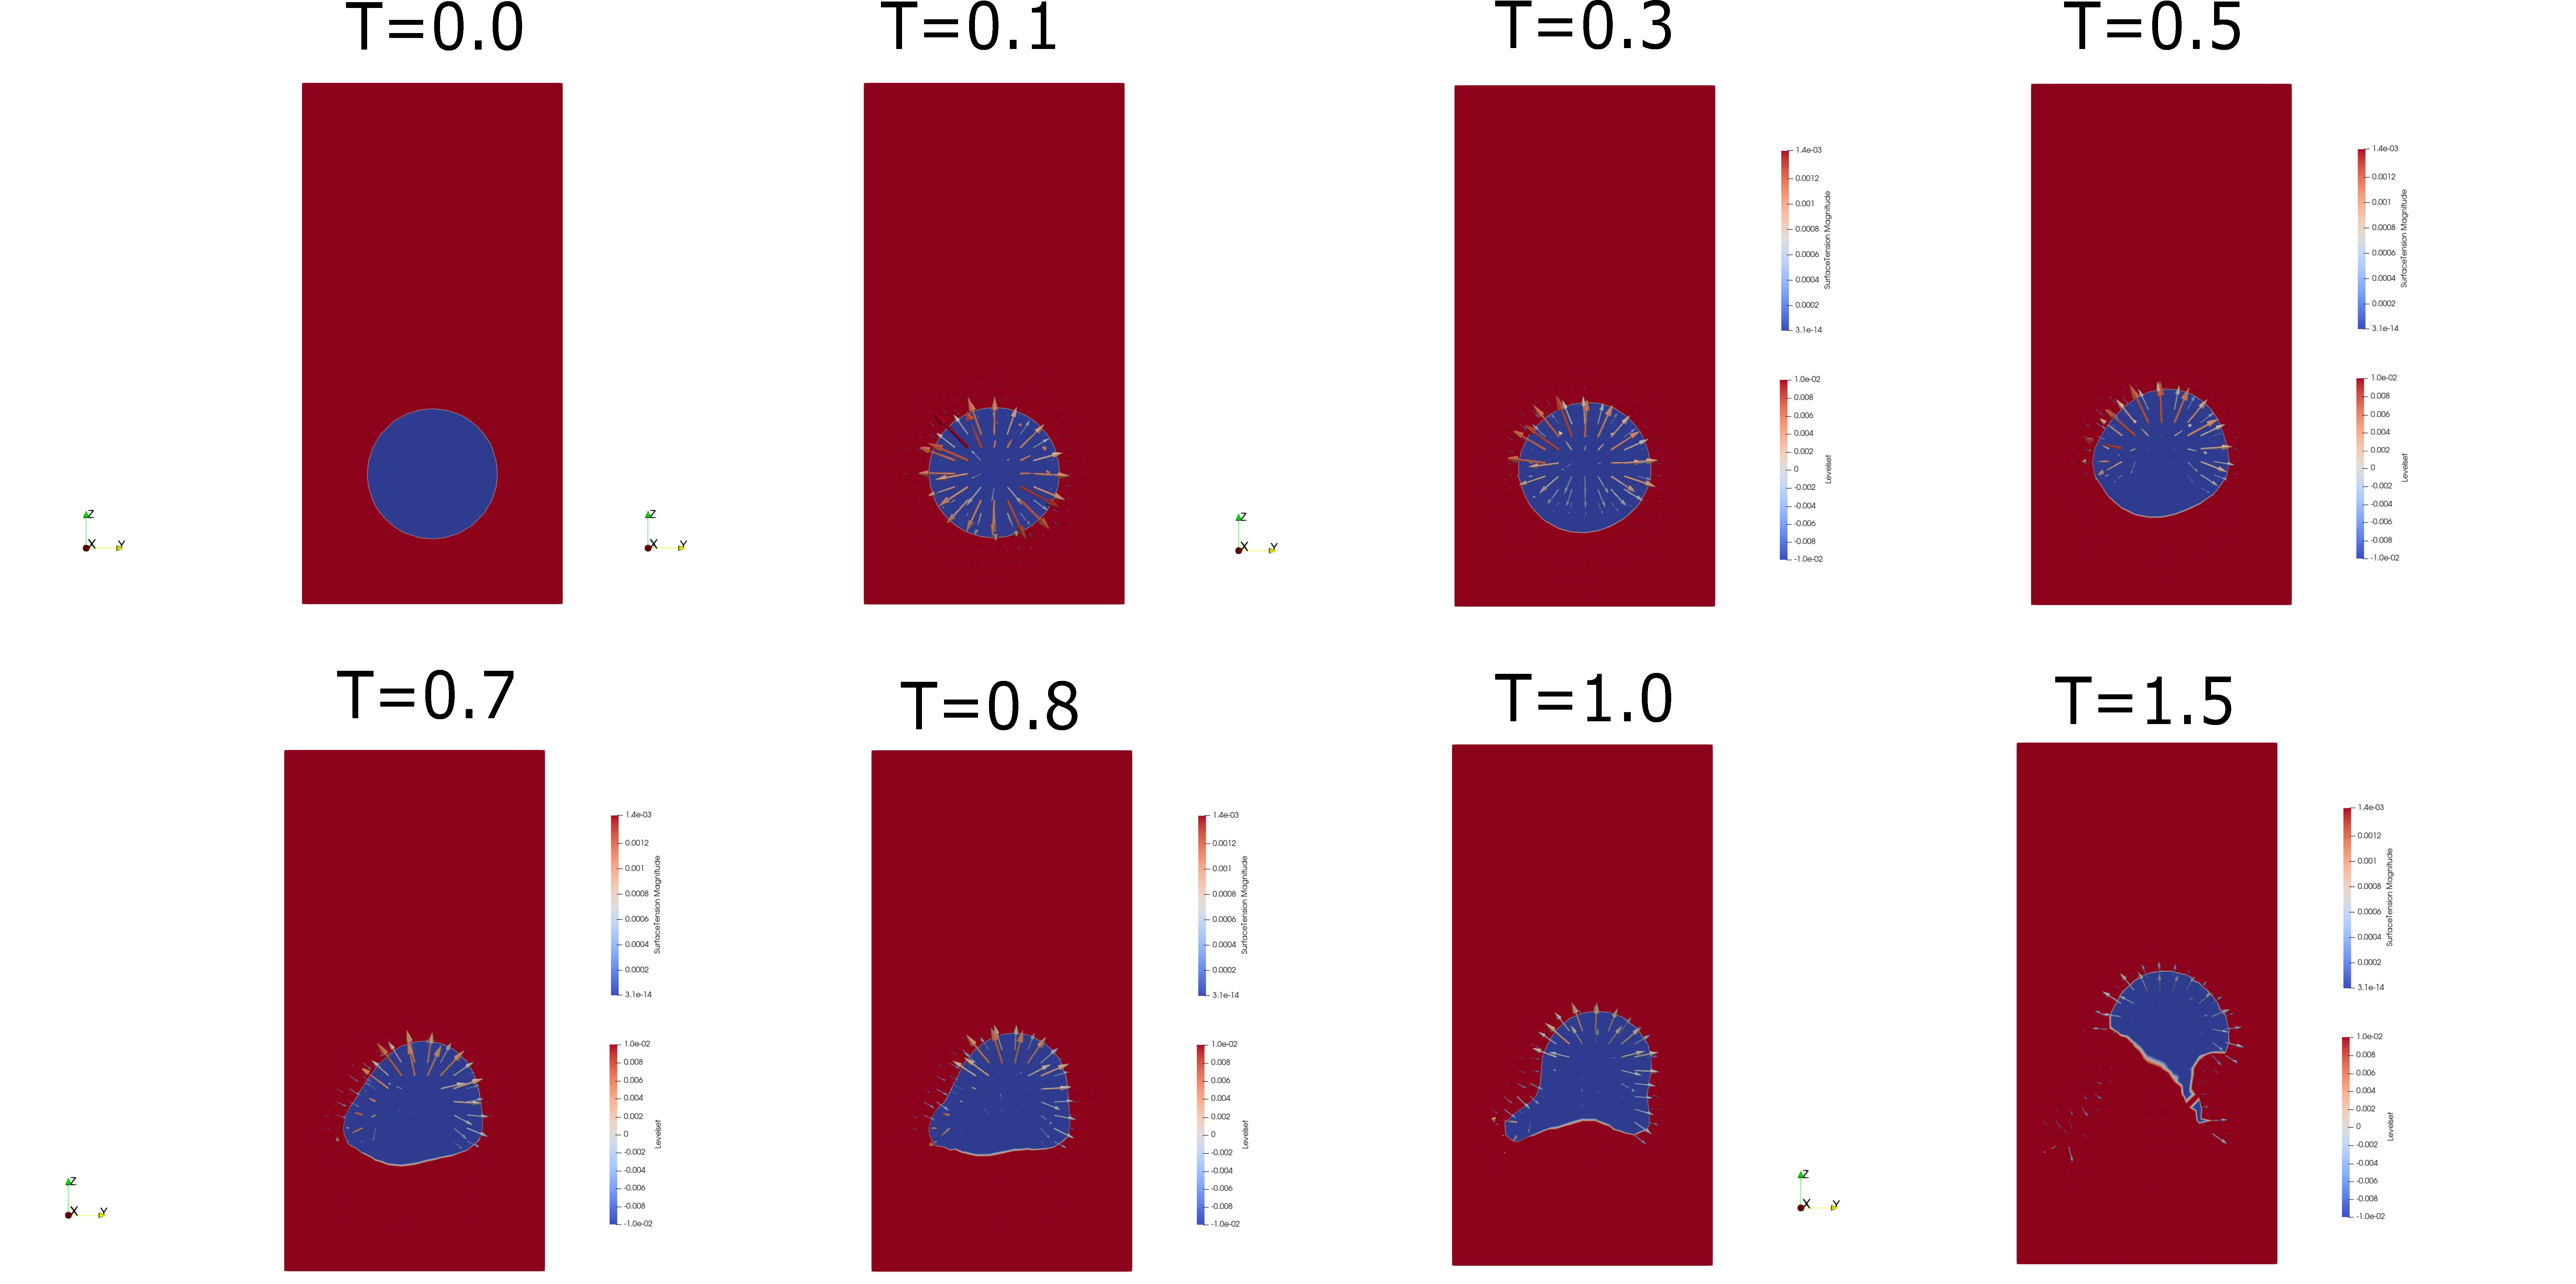
\includegraphics[width=18truecm]{pics/3d-bubble/result_sigma24_5.pdf}
	\caption{3次元気泡上昇流れのレベルセット関数の分布の時間変化($\sigma=24.5$、表面張力あり)。カラーバーの範囲は$-0.01$~$+0.01$として界面の位置を見やすくしている。}
	\label{fig:3d-bubble_result_sigma24.5}
\end{figure}

\begin{figure}[H]
	\centering
	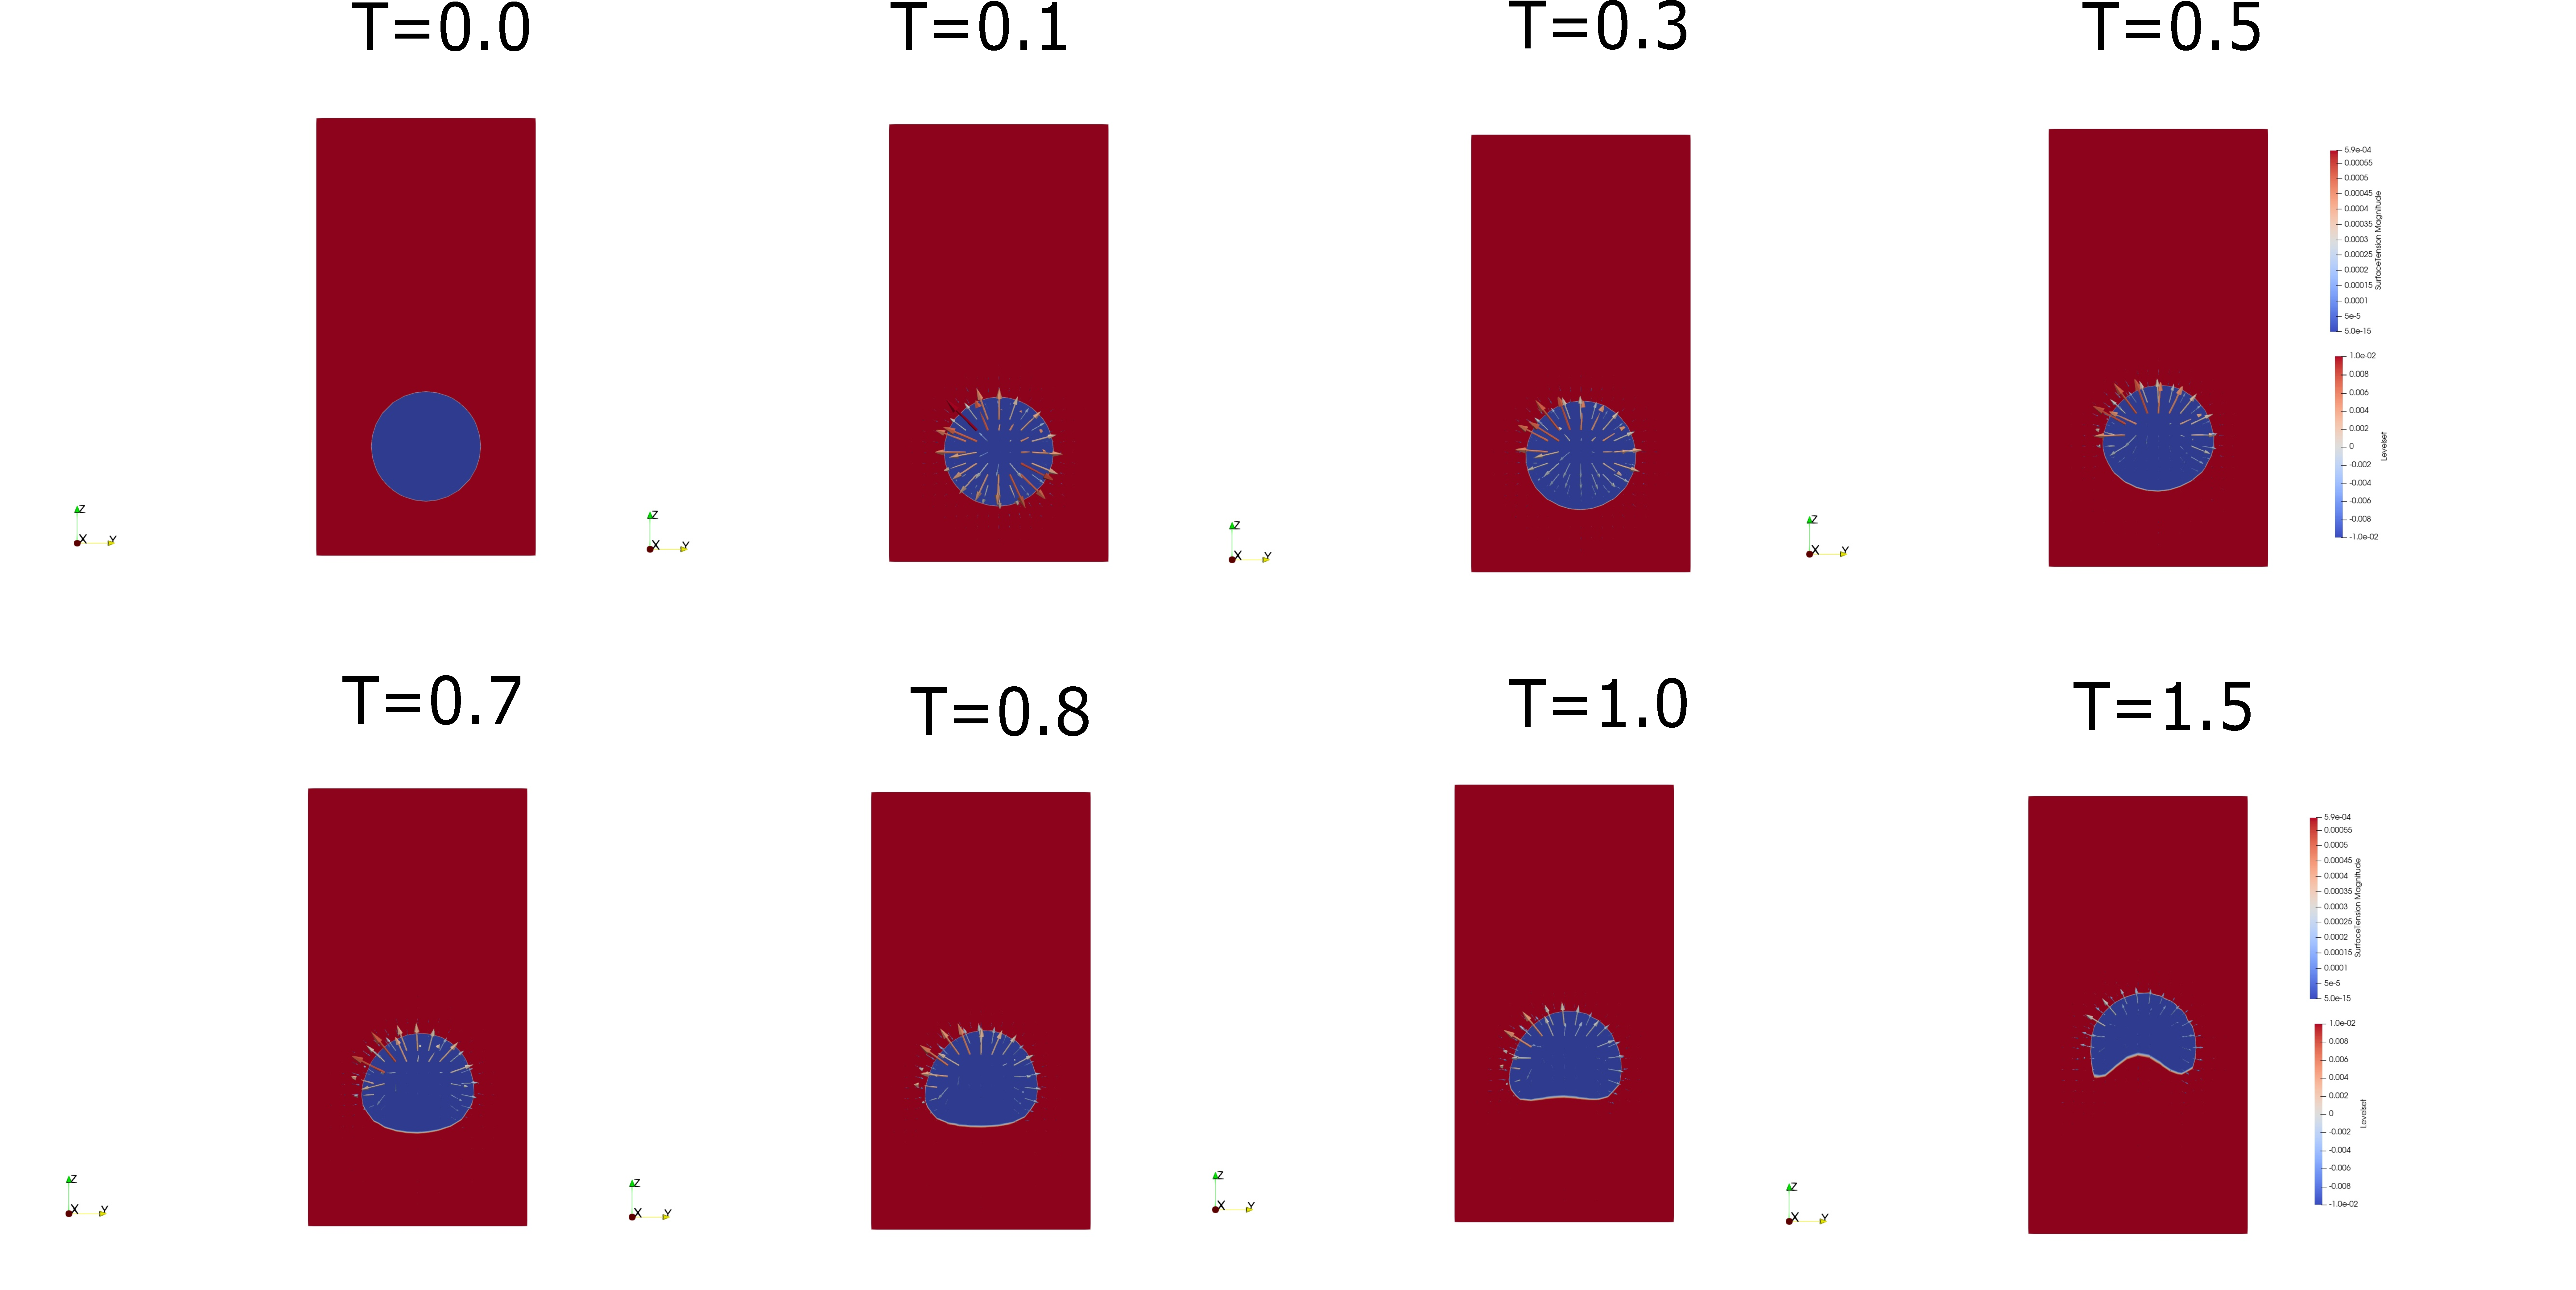
\includegraphics[width=18truecm]{pics/3d-bubble/result_sigma9_8.pdf}
	\caption{3次元気泡上昇流れのレベルセット関数の分布の時間変化($\sigma=9.8$、表面張力あり)。カラーバーの範囲は$-0.01$~$+0.01$として界面の位置を見やすくしている。}
	\label{fig:3d-bubble_result_sigma9.8}
\end{figure}

\begin{figure}[H]
	\centering
	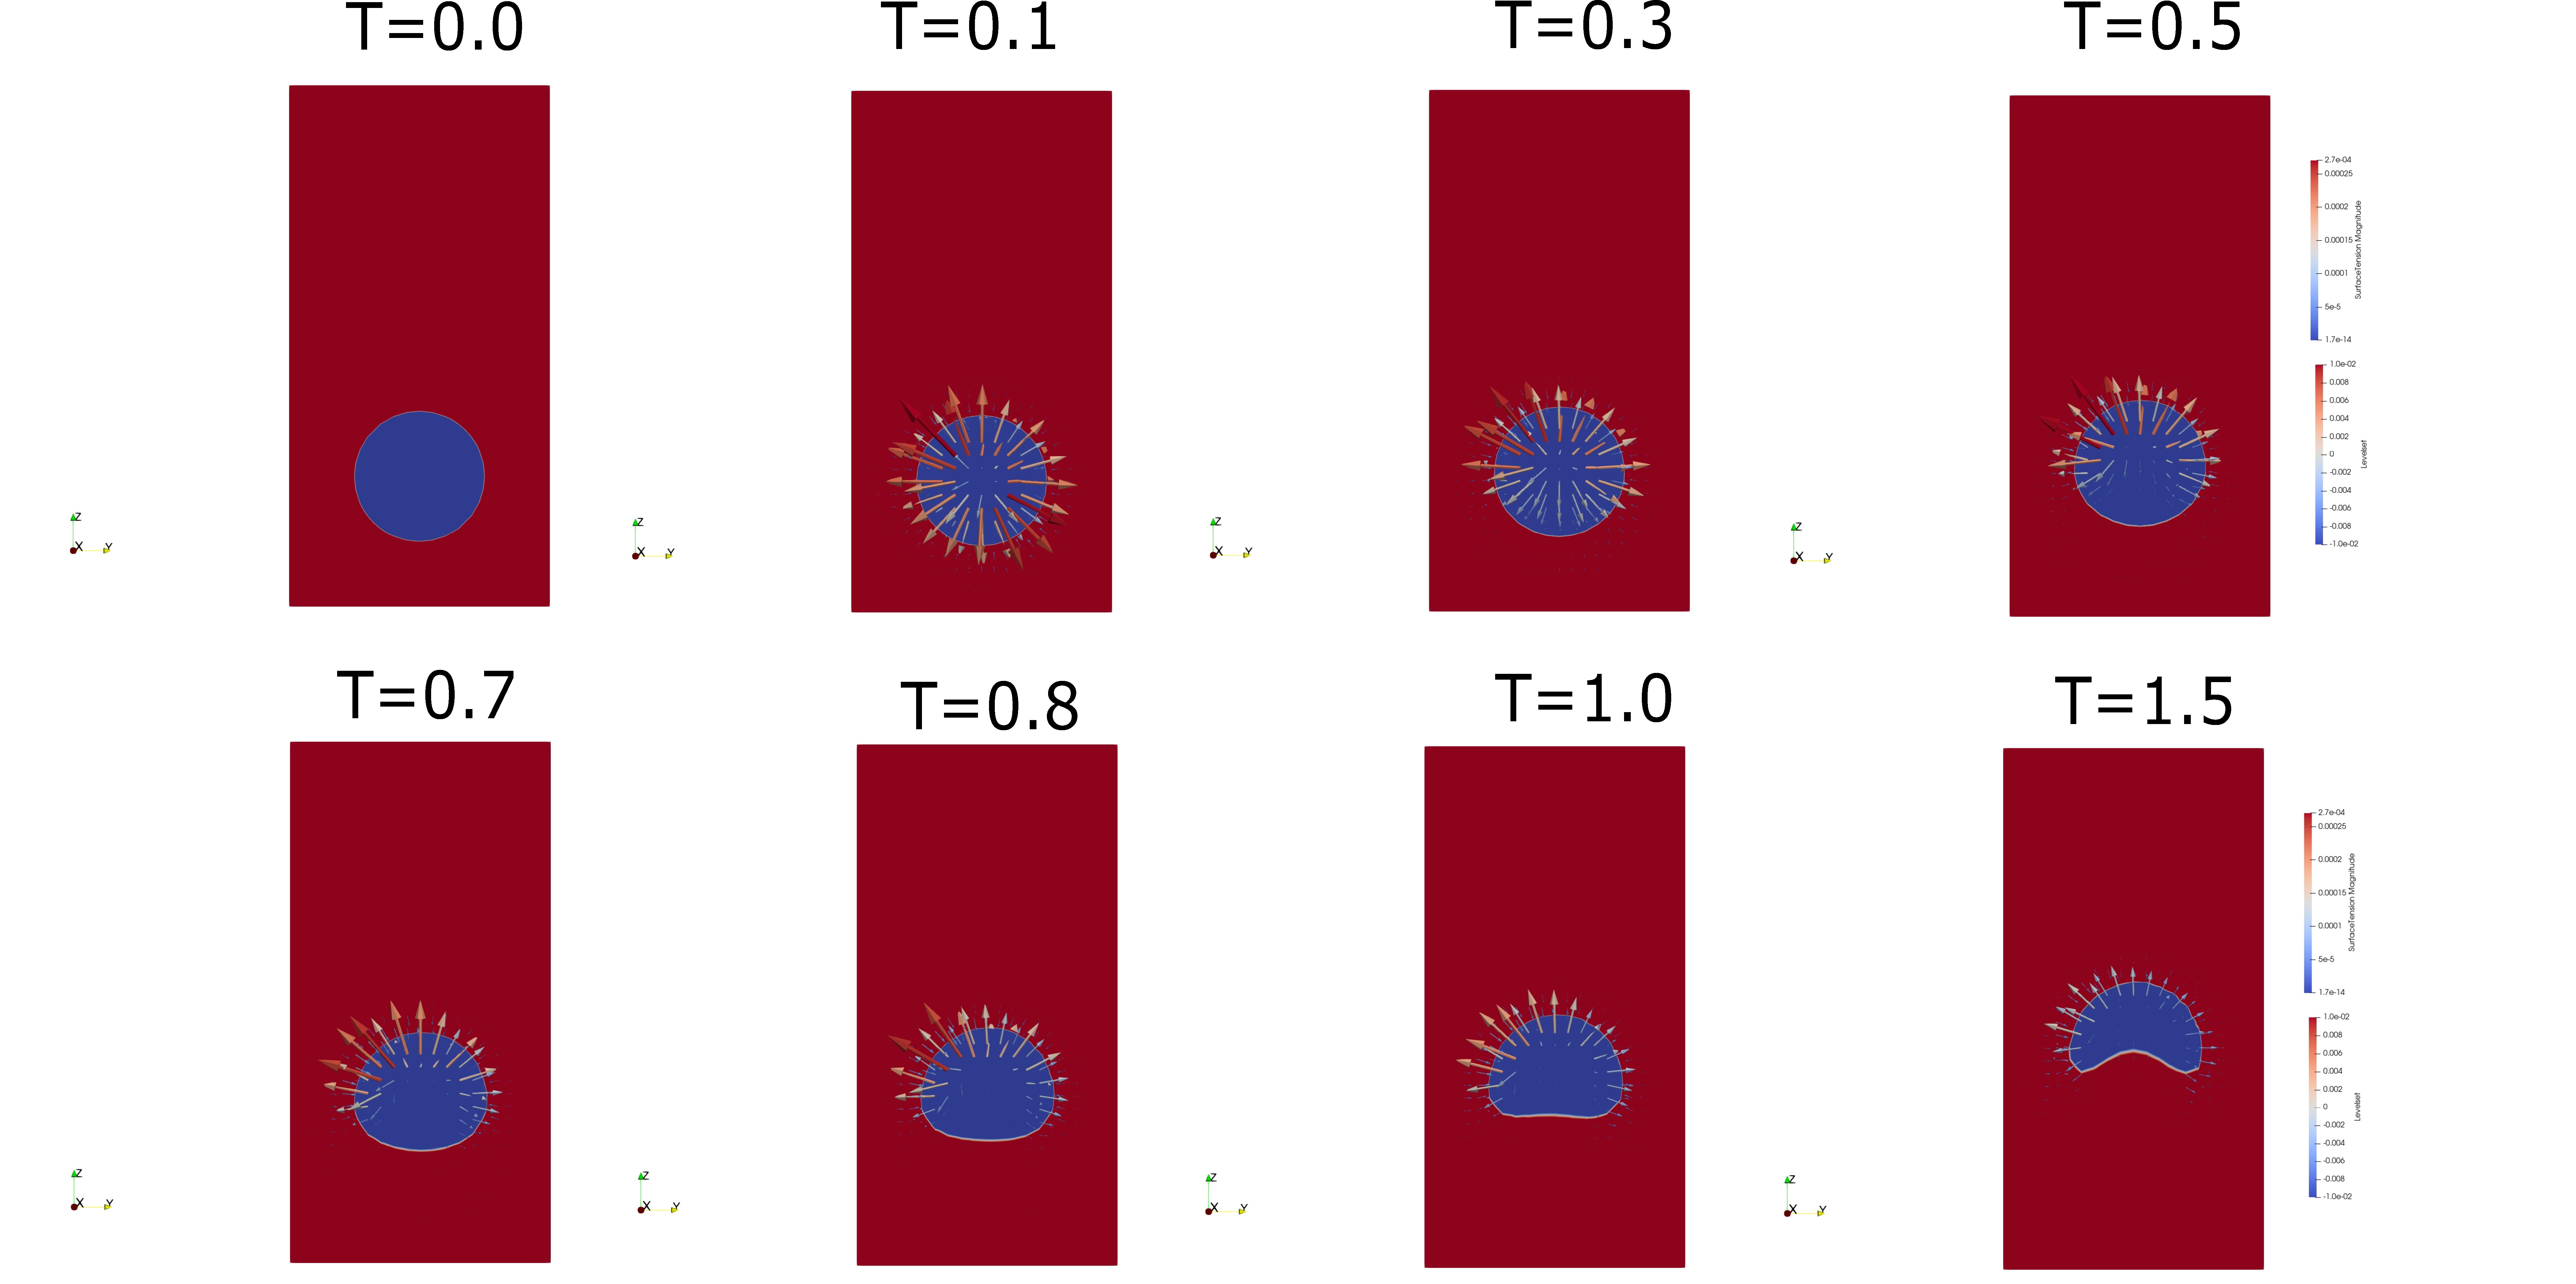
\includegraphics[width=18truecm]{pics/3d-bubble/result_sigma4_9.pdf}
	\caption{3次元気泡上昇流れのレベルセット関数の分布の時間変化($\sigma=4.9$、表面張力あり)。カラーバーの範囲は$-0.01$~$+0.01$として界面の位置を見やすくしている。}
	\label{fig:3d-bubble_result_sigma4.9}
\end{figure}

\begin{figure}[H]
	\centering
	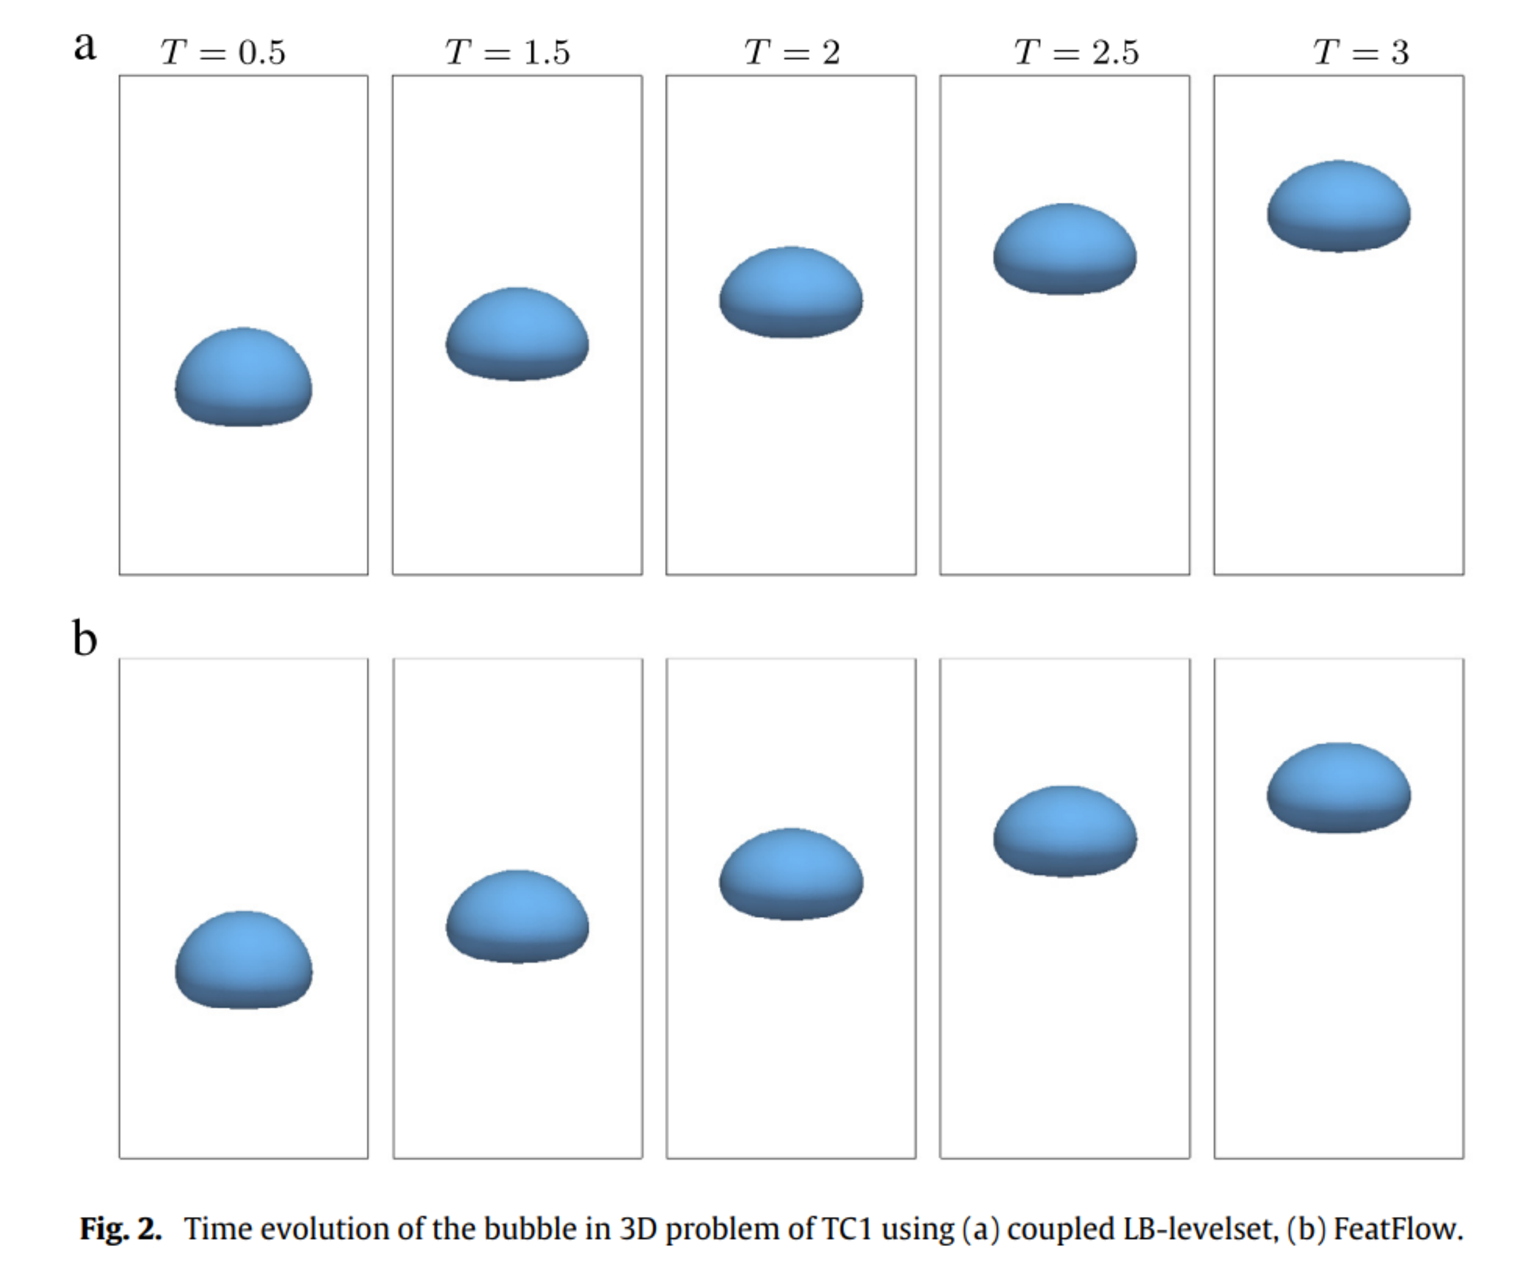
\includegraphics[width=10truecm]{pics/3d-bubble/result-ref.pdf}
	\caption{参考文献結果~\cite{Safi2017}}
	\label{fig:3d-bubble-result-ref}
\end{figure}

\begin{thebibliography}{99}
	\bibitem{Safi2017} Safi, M. A., Prasianakis, N. \& Turek, S. Benchmark computations for 3D two-phase flows: A coupled lattice Boltzmann-level set study. Comput. Math. Appl. 73, 520–536 (2017)
	\bibitem{Nagrath2003} Nagrath, S., Jansen, K. \& Lahey, R. T. Three Dimensional Simulation of Incompressible Two-phase Flows using a stabilized finite element method and level set approach. in vol. 56 KF.002 (2003)
	\bibitem{Matsumoto2006} 松本純一, 鈴木健 \& 手塚明. 気泡関数要素安定化法を用いた気液二相流解析. 混相流研究の進展 1, 181–188 (2006)
	\bibitem{Shi2019} Shi, J., Barriere, T., Liu, B. \& Cheng, Z. A simple and systematic scheme implemented in explicit FEM solver for surface tension effects in powder injection moulding process. Int. J. Mater. Form. 12, 123–134 (2019)
	\bibitem{Lo2005} Lo, D. C., Murugesan, K. \& Young, D. L. Numerical solution of three-dimensional velocity-vorticity Navier-Stokes equations by finite difference method. International Journal for Numerical Methods in Fluids vol. 47 1469–1487 Preprint at https://doi.org/10.1002/fld.822 (2005)
\end{thebibliography}

\end{document}

